\documentclass{emulateapj}
\bibliographystyle{apj}

%define general packages
\usepackage{epsfig}
\usepackage{rotating}
\usepackage{amsmath}
\usepackage{natbib}
\usepackage{footnote}
\usepackage{courier}

%internal short cuts
\def \HgA {H$\gamma_A$}
\def \Hbp {H$\beta ^\prime$}

\begin{document}

\title{PRIMUS: Galaxy Environment on the Quiescent Fraction Evolution at $z < 1$}
\author{
ChangHoon~Hahn\altaffilmark{1}, 
Michael~Blanton\altaffilmark{1}, 
Alison~Coil\altaffilmark{2}, 
Richard~Cool\altaffilmark{3}, 
Daniel Eisenstein\altaffilmark{4},
John Moustakas\altaffilmark{5}, 
Ken Wong\altaffilmark{6}, 
Guangtun Zhu\altaffilmark{7}
}
\altaffiltext{1}{Center for Cosmology and Particle Physics, Department of Physics, New York University, 4 Washington Place, New York, NY 10003}
\altaffiltext{2}{Center for Astrophysics and Space Sciences, Department of Physics, University of California, 9500 Gilman Dr., La Jolla, CA 92093}
\altaffiltext{3}{MMT Observatory, University of Arizona, 1540 E Second Street, Tucson AZ 85721}
\altaffiltext{4}{Harvard-Smithsonian Center for Astrophysics, 60 Garden Street, Cambridge, MA 02138}
\altaffiltext{5}{Department of Physics and Astronomy, Siena College, 515 Loudon Road, Loudonville, NY 12211}
\altaffiltext{6}{Steward Observatory, University of Arizona, 933 North Cherry Avenue, Tucson, AZ 85721} 
\altaffiltext{7}{Department of Physics and Astronomy, The Johns Hopkins University, 3400 North Charles Street, Baltimore, MD 21218} 
%%%%%%%%%%%%%%%%%%%%%%%%%%%%%%%%%%%%%%%%%%%%%%%%%%%%%%%%%%%%%%%%%%%%%%%%%%%%%%%%%%%%
% ABSTRACT
%%%%%%%%%%%%%%%%%%%%%%%%%%%%%%%%%%%%%%%%%%%%%%%%%%%%%%%%%%%%%%%%%%%%%%%%%%%%%%%%%%%%
\begin{abstract}
We investigate the effects of galaxy environment on the evolution of the quiescent fraction ($f_{\rm{Q}}$) from $z =0.8 $ to $ 0.0$ using spectroscopic redshifts and multi-wavelength imaging data from the PRism MUlti-object Survey (PRIMUS) and the Sloan Digitial Sky Survey (SDSS). Our stellar mass limited galaxy sample consists of $\sim 40000$ PRIMUS galaxies within $z = 0.2-0.8$ and $\sim 130,000$ SDSS galaxies within $z = 0.05-0.12$. We classify the galaxies as quiescent or star-forming based on an evolving specific star formation cut, and as low or high density environments based on fixed cylindrical aperture environment measurements on a volume-limited Environment Definition Population (from PRIMUS and SDSS). For quiescent and star-forming galaxies in low or high density environments, we examine the evolution of their stellar mass function (SMF) evolution. Then using the SMFs we compute the $f_{\rm{Q}}(\mathcal{M}_{*})$ and quantify the evolution of $f_{\rm{Q}}(\mathcal{M}_{*})$ within our redshift range. We find that in both low and high density environments the quiescent fraction increases with cosmic time. Moreover, we illustrate that galaxy populations in high density environments have significantly higher quiescent fractions than galaxy populations in low density environments. Furthermore, by comparing the quiescent fraction evolutions, we find that the quiescent fraction evolves noticeably more for galaxy populations in high density environments. These results suggest that quenching due to the environment has a moderate effect on the quiescent fraction evolution and provide constraints on quenching mechanisms in high density environments such as groups and clusters. 
\end{abstract}

%%%%%%%%%%%%%%%%%%%%%%%%%%%%%%%%%%%%%%%%%%%%%%%%%%%%%%%%%%%%%%%%%%%%%%%%%%%%%%%%%%%%
% INTRODUCTION
%%%%%%%%%%%%%%%%%%%%%%%%%%%%%%%%%%%%%%%%%%%%%%%%%%%%%%%%%%%%%%%%%%%%%%%%%%%%%%%%%%%%
\section{Introduction}
Galaxies, in their detailed properties, carry the imprints of their
surroundings, with a strong dependence of the quiescent fraction of
galaxies on their local environment (e.g. \citealt{hubble36a,
oemler74a, dressler80a, hermit96a, guzzo97a}; for a recent review see
\citealt{blanton09a}).  The strength of this dependence is itself a
strongly decreasing function of galaxy stellar mass; at the extreme,
the lowest mass ($<10^{9}$ $M_\odot$) galaxies are quenched only in
dense regions, and never in isolation (\citealt{geha12a}).  These
effects vary with redshift at least in the densest clusters, as
observed in the changing fraction of late-type spirals relative to the
field found in studies of the morphology-density relation
(\citealt{dressler84a, desai07a}).  Clearly understanding the
properties of galaxies in the present-day universe requires a careful
investigation of the role of environment, and how that role changes
over time.

Nevertheless, the evolution of the role of environment is a relatively
subtle effect and difficult to study.  Although history of galaxies
prior to $z\sim 1$ appears to have been one of rapid assembly, since
that time the galaxy population has continued to evolve, but less
dramatically. Although there are detectable changes in the population,
the major classes of galaxies existed at $z\sim 1$, in roughly the
same relative numbers as today (\citealt{bundy06a, borch06a,
taylor09a, Moustakas:2013aa}). Furthermore, at those redshifts we can also
detect the dependence of galaxy properties on environment, with lower
star-formation rate early-type galaxies populating the denser regions
(\citealt{cooper08a, patel09a, kovac10a}).

The most dramatic change in galaxy properties during the past eight
billion years has been a remarkable decline in the star-formation rate
of galaxies in the Universe (\citealt{hopkins06a}).  This decline
appears dominated by decreases in the rates of star-formation of
individual galaxies (\cite{Noeske:2007aa}). There is evidence that a
large fraction of the decline is associated with strongly
infrared-emitting starbursts (\citealt{bell05a, magnelli09a}).  The
decline does not appear to be due to the quenching of a large
fractions of the star-forming population, as reflected in observations
of the stellar mass function of quiescent and star-forming galaxies
(\citealt{Blanton:2006aa, bundy06a, borch06a, Moustakas:2013aa}).  These
findings leave little room for the participation of
environmentally-driven quenching in the global census of
star-formation.  As \citet{cooper08a} and others have pointed out,
because the environmental dependence of total star-formation rates at
fixed redshift is relatively small, environmentally effects are
unlikely to cause the overall star-formation rate decline.

Thus, the impact of environment on galaxy formation has to be
interpreted on top of the background of this overall decline affecting
galaxies in all environments. The most straightforward investigation
would directly determine the star-forming properties of galaxies as
a function of environment, stellar mass and redshift in a single,
consistently analyzed data set. This analysis can reveal how galaxies
are quenched in the universe over time, quantitatively establish the
contribution of environmental effects to the overall trends, and
reveal whether those trends happen equally in all environments.
However, such an analysis has not been done previously due to the lack
of sufficiently large samples. In this paper, we apply this approach
using the Prism Multi-object Survey (PRIMUS; \cite{Coil:2011aa}, 
\cite{Cool:2013aa}), the largest available redshift survey covering the epochs
between $0<z<1$.

In Section \ref{sec:sample} we present a brief description of the PRIMUS and SDSS data, our mass complete sample construction, and galaxy environment measurements. After dividing our galaxy sample into subsamples of star-forming or quiescent and high or low density environments, we compute and examine the evolution of the stellar mass functions for our subsamples. In Section \ref{sec:qf_const}, we calculate the quiescent fraction and compare the evolution of the quiescent fraction between high and low density environments. In Section \ref{sec:discussion} we discuss the trends observed in the stellar mass function and quiescent fraction evolution and discuss implications of the results on quenching mechanisms. Finally in Section \ref{sec:summary} we summarize our results. 

Throughout the paper we assume cosmology with $\Omega_{m} = 0.3, \Omega_{\Lambda} = 0.7$, and $H_0 = 70 \: \rm{km} \; \rm{s}^{-1} \rm{Mpc}^{-1}$.
%%%%%%%%%%%%%%%%%%%%%%%%%%%%%%%%%%%%%%%%%%%%%%%%%%%%%%%%%%%%%%%%%%%%%%%%%%%%%%%%%%%%
% SAMPLE SELECTION
%%%%%%%%%%%%%%%%%%%%%%%%%%%%%%%%%%%%%%%%%%%%%%%%%%%%%%%%%%%%%%%%%%%%%%%%%%%%%%%%%%%%
\section{Sample Selection} \label{sec:sample}
We are interested in quantifying the effects of galaxy environment on the evolution of the quenched fraction over the redshift range $0 < z < 1$. For our analysis, we require a sample with sufficient depth and robustness to probe the redshift range and to measure galaxy environment. PRIMUS with its $\sim 120,000$ spectroscopic redshifts provides a large data set at intermediate redshifts for our analysis. In addition, we anchor our analysis at intermediate redshifts with a low redshift sample derived from the Sloan Digital Sky Survey (\cite{York:2000aa}). 

In Section \ref{sec:primus} and Section \ref{sec:sdss} we provide a brief summary of the PRIMUS data and the SDSS data used for our sample selection. Then in Section \ref{sec:target} we define our stellar mass complete galaxy sample. Afterwards, in Section \ref{sec:sfq}, we classify our sample galaxies as quiescent or star-forming then calculate the environment using a volume-limited Environment Defining Population in Section \ref{sec:environment}. 
Finally in Section \ref{sec:edgeeffect}, we correct our galaxy sample and environment measurements for edge effects of the surveys. 

\begin{figure*}
    \begin{center}
        \leavevmode
        \epsscale{1.2}
	\plotone{fig_edp_sdss_z005_012_primus_z02_10_Mr_redshift.png}
        \caption{Absolute magnitude $M_{r}$ versus redshift for our mass complete galaxy sample (black squares) with the Environment Defining Population (red circles) plotted on top. Both samples are divided into redshift bins:$z \approx 0.05-0.12$, $0.2-0.4$, $0.4-0.6$, and $0.6-0.8$ (panels left to right). The lowest redshift bin ($z \approx 0.05-0.12$; leftmost panel) contain our galaxy sample and EDP selected from SDSS. The rest contain galaxies and EDP selected from PRIMUS. The redshift limits for the lowest redshift bin are empirically selected based on the bright and faint limits of SDSS galaxies. Stellar mass completeness limits, specified in Section \ref{sec:target}, are imposed on the galaxy population. Meanwhile, $M_{r}$ limits are applied to the EDP such that the number density in each panel are equivalent (Section \ref{sec:environment}).} \label{fig:targetEDP}
    \end{center}
\end{figure*}
%%%%%%%%%%%%%%%%%%%%%%%%%%%%%%%%%%%%%%%%%%%%%%%%%%%%%%%%%%%%%%%%%%%%%%%%%%%%%%%%%%%%
% PRIMUS
%%%%%%%%%%%%%%%%%%%%%%%%%%%%%%%%%%%%%%%%%%%%%%%%%%%%%%%%%%%%%%%%%%%%%%%%%%%%%%%%%%%%
\subsection{PRIMUS} \label{sec:primus}
At intermediate redshifts we use multiwavelength imaging and spectroscopic redshifts from PRIMUS, a faint galaxy survey with $\sim 120,000$ redshifts ($\sigma_z/(1+z) \approx 0.5 \%$) within the range $z \approx 0-1.2$. The survey was conducted using the IMACS spectrograph on the Magellan I Baade $6.5$ m telescope with a slitmask and low dispersion prism. For details on the PRIMUS observation methods such as survey design, targeting, and data summary, we refer readers to the survey papers (\citealt{Coil:2011aa, Cool:2013aa}). 

While the PRIMUS survey targeted seven distinct extragalactic deep fields for a total of $\sim 9 \; \rm{deg}^2$, we restrict our sample to five fields that have $GALEX$ and {\em Spitzer}/IRAC imaging (similar to the sample selection in \citealt{Moustakas:2013aa}). Four of these fields are a part of the {\em Spitzer} Wide-area Infrared Extragalactic Survey (SWIRE\footnote{http://swire.ipac.caltech.edu/swire/swire.html}): the European Large Area ISO Survey - South $1$ field (ELAIS-S1\footnote{http://dipastro.pd.astro.it/esis}), the Chandra Deep Field South SWIRE field (CDFS), and the XMM Large Scale Structure Survey field (XMM-LSS). The XMM-LSS consists of two separate but spatially adjacent fields: the Subaru/XMM-Newton DEEP Survey field (XMM-SXDSS\footnote{http://www.naoj.org/cience/SubaruProject/SDS}) and the Canadian-France-Hawaii Telescope Legacy Survey field (XMM-CFHTLS\footnote{http://www.cfht.hawaii.edu/Science/CFHLS}). Our fifth and final field is the Cosmic Evolution Survey (COSMOS\footnote{http://cosmos.astro.caltech.edu}) field. For all of our fields we have near-UV (NUV) and far-UV (FUV) photometry from the {\em GALEX} Deep Imaging Survey (DIS; \citealt{Martin:2005aa, Morrissey:2005aa}) as well as ground-based optical and {\em Spitzer}/IRAC mid-infrared photometric catalogs. \cite{Moustakas:2013aa} provides detailed descriptions of integrated flux calculations in the photometric bands for each of our fields. 

Finally, using the spectroscopic redshift and broad wavelength photometry we apply \texttt{iSEDfit}, a Bayesian SED modeling code, to calculate stellar masses and star formation rates (SFRs) for our sample galaxies (\citealt{Moustakas:2013aa}). \texttt{iSEDfit} uses the redshift and the observed photometry of the galaxies to determine the statistical likelihood of a large ensemble of generated model SEDs. The model SEDs are generated using Flexible Stellar Population Synthesis (FSPS) models (\citealt{Conroy:2010aa}) based on the \cite{Chabrier:2003aa} IMF, along with other prior parameters discussed in Section 4.1 and Appendix A of \cite{Moustakas:2013aa}. For the observed photometry, we use the {\em GALEX} FUV and NUV, the two shortest IRAC bands at $3.6$ and $4.5 \mu \rm{m}$ (the two longer-wavelength IRAC channels are excluded because \texttt{iSEDfit} does not model hot dust or polycyclic aromatic hydrocarbons emission lines), and the optical bands. 

\begin{table} %Subject to significant change based on the classification of environment
  \caption{Galaxy Subsamples}
  \label{tab:subsample}
  \begin{center}
    \leavevmode
    \begin{tabular}{l l l l l l l } \hline \hline              
    $z$ &$n_{\rm{env}}$        &Quiescent  &Star-forming  & $\mathcal{M}_{\rm{lim}}$ & $M_{\rm{r}, lim}$ \\ \hline 
$0.05-0.12$ &Low           &12859                       &14443                           \\
               &High            &18952                       &13387                           \\ 
                              &               &                       &                           \\ \hline
$0.2-0.4$      &Low           &1158                    &3445                           \\
               &High            &817                    &1531                           \\
               &               &                       &                           \\ \hline
$0.4-0.6$      &Low           &1315                       &3390                           \\
               &High            &848                       &1499                           \\
               &               &                       &                           \\ \hline
$0.6-0.8$      &Low           &1158                       &2303                           \\
               &High            &900                       &1275                           \\
               &               &                       &                           \\ \hline
  \multicolumn{4}{l}{}                                             \\       
    \end{tabular} \par
    \end{center}
%    \bigskip 
    {\bf Notes}: Number of galaxies in the mass complete subsamples derived in Section \ref{sec:sample}. The subsamples are classified based on environment $n_{\rm{env}}$ and star formation rate (star-forming or quiescent). The lowest redshift bin is derived from SDSS; the rest are from PRIMUS. 
    \bigskip
\end{table}

%%%%%%%%%%%%%%%%%%%%%%%%%%%%%%%%%%%%%%%%%%%%%%%%%%%%%%%%%%%%%%%%%%%%%%%%%%%%%%%%%%%%
% SDSS-GALEX
%%%%%%%%%%%%%%%%%%%%%%%%%%%%%%%%%%%%%%%%%%%%%%%%%%%%%%%%%%%%%%%%%%%%%%%%%%%%%%%%%%%%
\subsection{SDSS-GALEX} \label{sec:sdss}
At low redshifts, we use spectroscopic redshifts and $ugriz$ photometry from the SDSS Data Release 7 (DR7; \citealt{Abazajian:2009aa}). More specifically we select galaxies from the New York University Value-Added Galaxy Catalog (hereafter VAGC) that satisfy the main sample criterion and have galaxy extinction corrected Petrosian magnitudes $14.5 < r < 17.6$ and spectroscopic redshifts within $0.01 < z < 0.2$ (\citealt{Blanton:2005aa}). We further restrict the VAGC sample to only galaxies with medium depth observations with total exposure time greater than $1 \; \rm{ks}$ from {\em GALEX} Release 6. This leaves $167,727$ galaxies. 

Next, we use the MAST/CasJobs\footnote{http://galex.stsci.edu/casjobs} interface and a $4''$ diameter search radius, to obtain the NUV and FUV photometry for the SDSS-{\em GALEX} galaxies. For optical photometry, we use the $ugriz$ bands from the SDSS \texttt{model} magnitudes scaled to the $r$-band \texttt{cmodel} magnitude. These photometric bands are then supplemented with integrated $JHK_s$ magnitudes from the 2MASS Extended Source Catalog (XSC; \citealt{Jarrett:2000aa}) and with photometry at $3.4$ and $4.6 \mu \rm{m}$ from the WISE All-Sky Data Release\footnote{http://wise2.ipac.caltech.edu/docs/release/allsky}. Further details regarding the SDSS-{\em GALEX} sample photometry can be found in Section 2.4 of \cite{Moustakas:2013aa}. As previously done on the PRIMUS data in Section \ref{sec:primus}, we use \texttt{iSEDfit} to obtain the stellar masses and star formation rates for the SDSS-{\em GALEX} sample. 

While the SDSS-{\em GALEX} data discussed above is derived from VAGC Data Release 7, since the release of the catalog, there have been significant improvements in the photometry. Notably, \cite{Blanton:2011aa} find that the background subtractions in SDSS Data Release 7 has a size dependent bias in the galaxy fluxes. In addition \cite{Bernardi:2013aa} find that the luminosity, and ultimately stellar mass, is underestimated when they are derived from the SDSS \texttt{cmodel} magnitudes in comparison to \texttt{PyMorph} single-S\'{e}rsic and Sersic-Exponential fits to the surface brightness profiles. 

In order to quantify the effects of these photometric underestimations in our analysis, we replace our SDSS fluxes in the $ugriz$ band with $ugriz$ fluxes from the NASA-Sloan Atlas (NSA) catalog, which incorporate the improved background subtraction presented in \cite{Blanton:2011aa} and uses single-Seric fit fluxes rather than the standard SDSS \texttt{cmodel} fluxes. Using the ratio of the luminosity derived from the improved photometry over the luminosity derived from the standard VAGCVAGC photometry, we apply a preliminary correction to the stellar mass values obtained from \texttt{iSEDfit} assuming a consistent mass-to-light ratio. This mass correction leads to a significant increase in the stellar mass function for $\mathcal{M} > 10^{11} \mathcal{M}_{\odot}$; however, the effect of the mass correction was negligible for the quiescent fraction evolution results. As a result, we do not discuss the issues with photometric measurements any further in this paper. The effects of the discussed photometry methods on the luminosity function and stellar mass function will be examined in detail in future work. 
%%%%%%%%%%%%%%%%%%%%%%%%%%%%%%%%%%%%%%%%%%%%%%%%%%%%%%%%%%%%%%%%%%%%%%%%%%%%%%%%%%%%
% GALAXY SAMPLE
%%%%%%%%%%%%%%%%%%%%%%%%%%%%%%%%%%%%%%%%%%%%%%%%%%%%%%%%%%%%%%%%%%%%%%%%%%%%%%%%%%%%
\subsection{Galaxy Sample} \label{sec:target} 
\begin{figure*}
  \begin{center}
    \leavevmode
    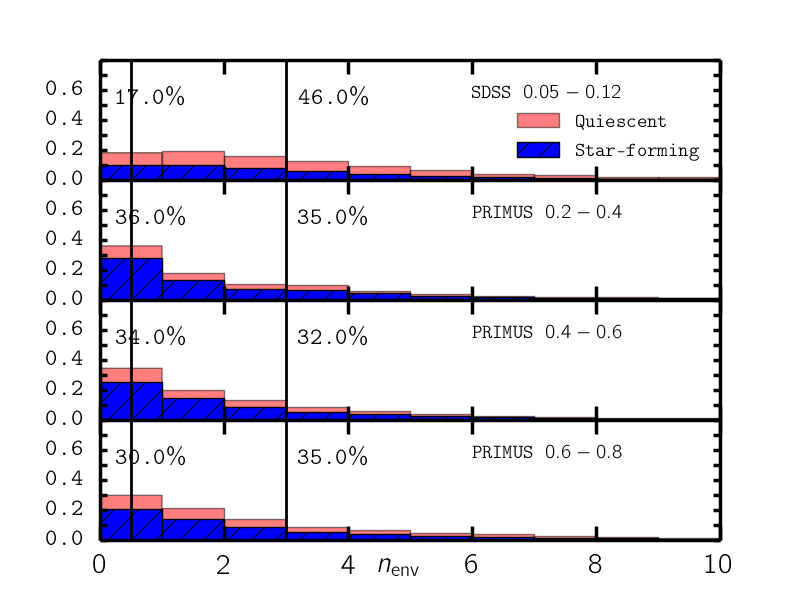
\epsfig{file=fig_envcount_cylr2h25_thresh75_sdss_z0_05_0_12_primus_z0_21_0_lowenv0_5_highenv3_0_primuszerr_masslimit_edgecut_histogram.png, height=0.5\textwidth}
     \caption{Normalized distribution of environment measurements ($n_{\rm{env}}$) for our mass complete galaxy sample within the edges. The star-forming galaxies contribution to the distribution is colored blue and diagonally patterned. The contribution from quiescent galaxies is colored in red. Each redshift panel is divided into three sections of by the environment classification cutoffs (vertical black lines): low density environment $n_{\rm{env}} < 0.5$ and high density environment $n_{\rm{env}} > 3.0$. The percentages of the redshift bin contained in the environment classifications are presented above the distribution. For example at $0.2 < z < 0.4$, $56.0 \%$ of galaxies in the redshift bin have low density environments while $29.0\%$ of galaxies in the redshift bin have high density environments. }      \label{fig:envcount}
    \end{center}
\end{figure*}

From the low redshift SDSS-{\em GALEX} and intermediate redshift PRIMUS data, in this section, we define our mass complete galaxy sample. We begin by imposing the parent sample selection criteria from \cite{Moustakas:2013aa}. More specifically, we take the statistically complete {\em primary} sample from the PRIMUS data (\citealt{Coil:2011aa}) and impose magnitude limits on optical selection bands as specified in \cite{Moustakas:2013aa} Table 1. These limits are in different optical selection bands and have distinct values for the five PRIMUS target fields. We then exclude stars and broad-line AGN to only select objects spectroscopically classified as galaxies, with high-quality spectroscopic redshifts ($Q \geq 3$). Lastly, we impose a redshift range of $ 0.2 < z < 0.8$ for the PRIMUS galaxy sample, where $ z > 0.2$ is selected due to limitations from sample variance and $ z < 0.8$ is selected due to the lack of sufficient statistics in subsamples defined below. 

For the PRIMUS objects that meet the above criteria, we assign statistical weights (described in \citealt{Coil:2011aa} and \citealt{Cool:2013aa}) in order to correct for targeting incompleteness and redshift failures. The statistical weight, $w_i$, for each galaxy is given by
\begin{equation}
w_{i} = (f_{\rm{target}} \times f_{\rm{collision}} \times f_{\rm{success}})^{-1},
\end{equation}
as in Equation (1) in \cite{Moustakas:2013aa}. Since we are ultimately interested in a mass complete galaxy sample to derive SMFs and QFs, next we impose stellar mass completeness limits to our galaxy sample. 

Stellar mass completeness limits for a magnitude-limited survey such as PRIMUS are functions of redshift, the apparent magnitude limit of the survey, and the typical stellar mass-to-light ratio of galaxies near the flux limit. As in \cite{Moustakas:2013aa}, we follow \cite{Pozzetti:2010aa} to empirically determine the stellar mass completeness limits. For each of the target galaxies we compute $\mathcal{M}_{\rm{lim}}$ using $\rm{log} \; \mathcal{M}_{\mathrm{lim}} = \mathrm{log} \; \mathcal{M} + 0.4 (m - m_{\mathrm{lim}})$, where $\mathcal{M}$ is the stellar mass of the galaxy in $\mathcal{M_{\odot}}$, $\mathcal{M}_{\rm{lim}}$ is the stellar mass of each galaxy if its magnitude was equal to the survey magnitude limit, $m$ is the observed apparent magnitude in the selection band, and $m_{\rm{lim}}$ is the magnitude limit for our five fields. We construct a cumulative distribution of $\mathcal{M}_{\rm{lim}}$ for the $15\%$ faintest galaxies in $\Delta z=0.04$ bins. In each of these redshift bins, we calculate the minimum stellar mass that includes $95 \%$ of the galaxies. Separately for quiescent and star-forming galaxies, we fit quadratic polynomials to the minimum stellar masses versus redshift (star-forming or quiescent classification is described in the following section). Finally, we use the polynomials to obtain the minimum stellar masses at the center of redshift bins, $0.2-0.4$, $0.4-0.6$, and $0.6-0.8$, which are then used as PRIMUS stellar mass completeness limits.

For the low redshift portion of our galaxy sample, we start by limiting the SDSS-{\em GALEX} data to objects within $0.05 < z < 0.12$, a redshift range later imposed on the volume-limited Environment Defining Population (Section \ref{sec:environment}). To account for the targeting incompleteness of the SDSS-{\em GALEX} sample, we use the statistical weight estimates provided by the NYU-VAGC catalog. Furthermore, we determine a uniform stellar mass completeness limit of $10^{10.2} \mathcal{M}_{\odot}$ above the stellar mass-to-light ratio of the SDSS-{\em GALEX} data within the imposed redshift limits. We then apply this mass limit in order to obtain our mass-complete galaxy sample at low redshift. 

We now have a stellar mass complete sample derived from SDSS-{\em GALEX} and PRIMUS data. Since our sample is derived from two different surveys, we account for the disparity in the redshift uncertainty. While PRIMUS provides a large number of redshifts out to $z = 1$, due to using a prism instead of a grating, the uncertainties are significantly larger ($\sigma_{z}/(1+z) \approx 0.5 \%$) than that of the SDSS-{\em GALEX} redshifts. In order to have comparable environment measures throughout our redshift range, we apply PRIMUS redshift uncertainties to our galaxy sample selected from SDSS-{\em GALEX}. For each SDSS-{\em GALEX} galaxy, we adjust its redshift by randomly sampling a Gaussian distribution with standard deviation $\sigma = 0.005 (1+z_{\rm{SDSS}-GALEX})$, where $z_{\rm{SDSS}-GALEX}$ is the redshift of the galaxy. 

We present the absolute magnitude ($M_{r}$) versus redshift for the galaxy sample (black squares) in Figure \ref{fig:targetEDP}. The left-most panel corresponds to the sample derived from the SDSS-{\em GALEX} data and the rest correspond to the target sample derived from the PRIMUS data divided in bins with $\Delta z \sim 0.2$. 
%%%%%%%%%%%%%%%%%%%%%%%%%%%%%%%%%%%%%%%%%%%%%%%%%%%%%%%%%%%%%%%%%%%%%%%%%%%%%%%%%%%%
% CLASSIFYING QUIESCENT AND STAR-FORMING GALAXIES
%%%%%%%%%%%%%%%%%%%%%%%%%%%%%%%%%%%%%%%%%%%%%%%%%%%%%%%%%%%%%%%%%%%%%%%%%%%%%%%%%%%%
\subsection{Classifying Quiescent and Star-Forming Galaxies} \label{sec:sfq}
We now classify our mass complete galaxy sample into quiescent or star-forming using an evolving cut based on specific star-formation rate utilized in \cite{Moustakas:2013aa} Section 3.2. This classification method uses the star-forming (SF) sequence, which is the correlation between star-formation rate (SFR) and stellar mass in star-forming galaxies observed at least until $z \sim 2$ (\citealt{Noeske:2007aa}). The PRIMUS sample displays a well-defined SF sequence within the redshift range of our galaxy sample. Using the power-law slope for the SF sequence from \cite{Salim:2007aa} (SFR $\propto \mathcal{M}^{0.65}$) and the minimum of the quiescent/star-forming bimodality, determined empirically, we obtain the following equation to classify the target galaxies (Equation 2 in \citealt{Moustakas:2013aa}):
\begin{equation}
\rm{log}(\rm{SFR}_{\rm{min}}) = -0.49 + 0.64 \rm{log}(\mathcal{M} - 10) +1.07(z-0.1), 
\end{equation} \label{eq:qsfclass} 
where $\mathcal{M}$ is the stellar mass of the galaxy. If the target galaxy SFR and stellar mass lie above Equation \ref{eq:qsfclass} we classify it as star-forming; if below, as quiescent (\citealt{Moustakas:2013aa} Figure 1.).

\begin{figure*}
  \begin{center}
    \leavevmode
    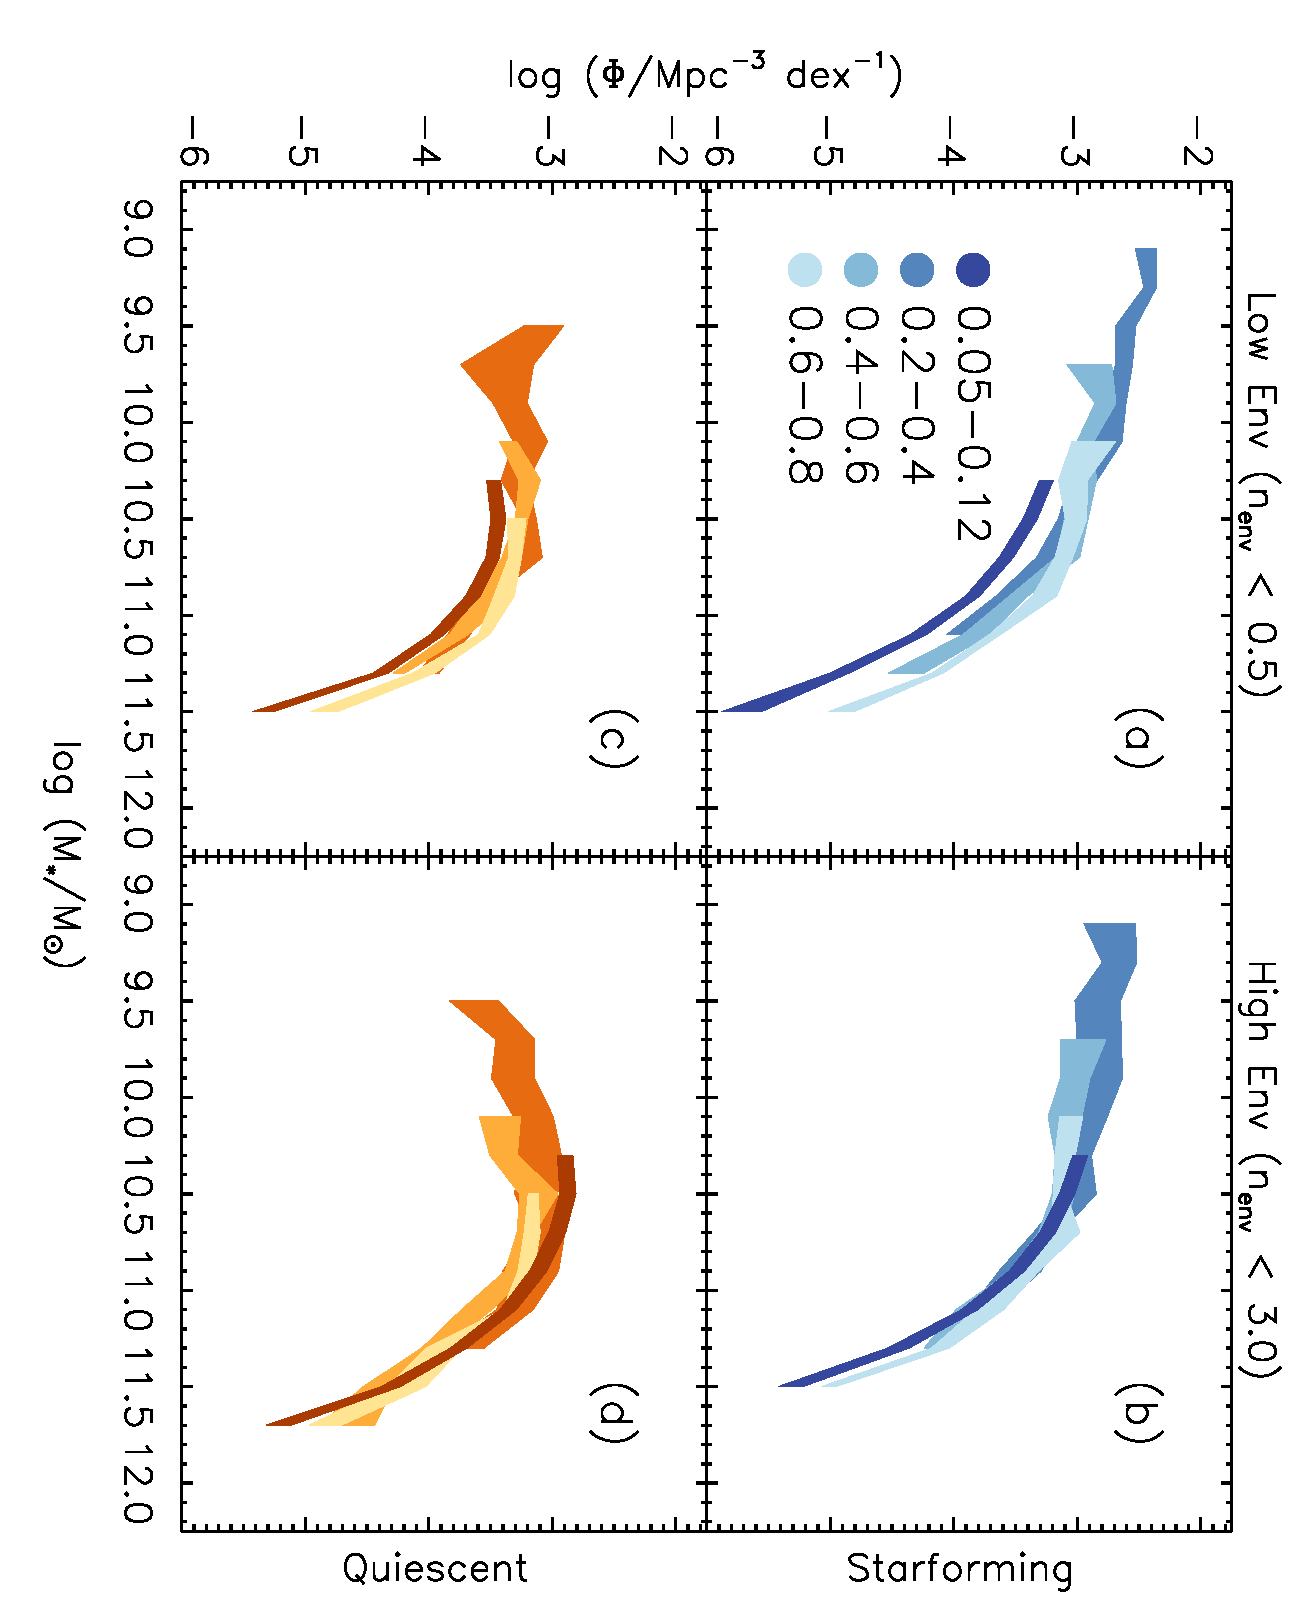
\epsfig{file=fig_smf_cylr2h25_thresh75_bin0_20_sdss_z0_05_0_12_primus_z0_2_1_0_2envbin_lowenv0_5_highenv3_0_lit_primuszerr.eps, height=0.75\textwidth,angle=90}
     \caption{Evolution of stellar mass functions of star-forming (top) and quiescent (bottom) target galaxies in 
low (left) and high (right) environments from redshift range $z=0-0.8$. The environment of each galaxy  
was calculated using a cylindrical aperture size of $R=2 \: \rm{Mpc}$ and $H=25 \: \rm{Mpc}$ and  
classification based on the cut-offs specified in Table \ref{tab:aperture}. The SMFs use mass bins of 
width $\Delta \rm{log}(\mathcal{M}/\mathcal{M}_{\odot})=0.25$. In each panel we use shades of blue 
(star-forming) and orange (quiescent) to represent the SMF at different redshift, higher redshifts being
progressively lighter.}      \label{fig:smf}
    \end{center}
\end{figure*}
%%%%%%%%%%%%%%%%%%%%%%%%%%%%%%%%%%%%%%%%%%%%%%%%%%%%%%%%%%%%%%%%%%%%%%%%%%%%%%%%%%%%
% GALAXY ENVIRONMENT
%%%%%%%%%%%%%%%%%%%%%%%%%%%%%%%%%%%%%%%%%%%%%%%%%%%%%%%%%%%%%%%%%%%%%%%%%%%%%%%%%%%%
\subsection{Galaxy Environment} \label{sec:environment}
We define the environment of a galaxy as the number of neighboring Environment Defining Population galaxies (defined below) within a fixed aperture centered around it. We use a fixed aperture measurement of environment in order to probe environment on the halo scale, as \cite{Muldrew:2012aa} finds in their comparison of different environment definition using simulations. 

For our aperture, we use a cylinder of dimensions: $R_{\rm{ap}} = 2 \; h^{-1} \rm{Mpc}$ and $H_{\rm{ap}} = 25 \; h^{-1}\rm{Mpc}$. Though spherical apertures are often used in literature (e.g. \citealt{Croton:2005aa}), we use a cylindrical aperture in order to account for the PRIMUS redshift errors and redshift space distortions (i.e. ``Finger of God" effect). \cite{Cooper:2005aa} finds that $\pm 1000 \; \rm{km} \; \rm{s^{-1}}$ optimally reduces the effects of redshift space distortions. The PRIMUS redshift uncertainty at $z \sim 0.7$ corresponds to $\sigma_z < 0.01$, so our aperture height choice of $25 \; \rm{Mpc}/h$ accounts for both of these effects. Our choice of cylinder radius was motivated by scale dependence analyses in literature (\citealt{Blanton:2006aa, Wilman:2010aa, Muldrew:2012aa}), which suggest that galactic properties such as color and quenched fractions are dependent on halo-scale properties such as host dark matter halo mass. \cite{Wilman:2010aa}, which uses environment defined by annuli of different radii, find positive correlation for quenched fraction and color on scales $< 1 \; \rm{Mpc}$ and anti-correlation on scales $> 3 \; \rm{Mpc}$. Our choice of $2 \rm{Mpc}/h$ provides sufficient sample size of galaxies in dense environments, for robust statistics, while tracing galactic properties within the halo scale. 

%When we extend our analysis to cylindrical apertures with $R_{\rm{ap}} = 1 \; \rm{Mpc}/h$, we find that the change does not qualitatively change our results (difference in $f_{Q} < 0.05$). 
%Similar fixed aperture methods have also been used in \cite{Croton:2005aa} for galaxies in the 2dF Galaxy Redshift 
%Survey (\cite{Colless:2003aa}) and in \cite{Muldrew:2012aa} for a mock galaxy catalogue generated from embedding 
%galaxies onto the Millenium Dark Matter Simulation (\cite{Springel:2005aa}). 

Before we measure the environment for our galaxy sample, we first construct a volume limited Environment Defining Population (EDP) with absolute magnitude cut-offs ($M_{r}$) at redshift bin of $\Delta z \sim 0.2$. The $M_{r}$ cut-offs for the EDP are selected such that the cumulative number density over $M_{r}$ for all redshift bins are equal. In addition to providing a reasonable comparison of environment measurements for wide redshift range, we make this choice in order to construct an EDP that contains similar galaxy populations through the redshift range (i.e. accounts for the progenitor bias). As \cite{Behroozi:2013aa} and \cite{Leja:2013aa} find in their analysis of the cumulative number density method, though it does not precisely account for the scatter in mass accretion or galaxy-galaxy mergers, it provides a reasonable means to compare galaxy populations over a wide range of cosmic time. 

In constructing the EDP for the PRIMUS (hereafter PRIMUS EDP) we use the same PRIMUS data used to select our galaxy sample (described in Section \ref{sec:target}). We again restrict the PRIMUS galaxies to $0.2 < z < 0.8$ and divide them into bins of $\Delta z = 0.2$. Before we consider the cumulative number densities in the redshift bins, we first determine the $M_r$ limit for the highest redshift bin ($0.6-0.8$) by examining the $M_{r}$ distribution with bin size $\Delta M_{r} = 0.25$ and select $M_{r,\rm{lim}}$ near the peak of the distribution where bins with $M_{r} > M_{r,\rm{lim}}$ have fewer galaxies than the bin at $M_{r, \rm{lim}}$. We conservatively choose $M_{r, \rm{lim}}(0.6 < z < 0.8)$ to be $M_{r} = -20.75$. Then for the lower redshift bins, we impose absolute magnitude limits ($M_{r,\rm{lim}}$) such that the cumulative number density, calculated with the galaxy statistical weights, of the bin ordered by $M_{r}$ is equal to the cumulative number density of the highest redshift bin at $M_{r, \rm{lim}}(0.6 < z < 0.8) = -20.75$. 

For the EDP of the SDSS-{\em GALEX} galaxy sample (hereafter SDSS EDP), we do not use the SDSS-{\em GALEX} parent data, which uses the geometry of the combined angular selection function of the VAGC and {\em GALEX} (Section \ref{sec:sdss}). Instead, since FUV, NUV values are not necessary for the EDP, we extend the parent data of the SDSS EDP to the entire NYU VAGC, including galaxies outside of the {\em GALEX} window function. Furthermore, we impose a redshift range of $0.05-0.12$ on the SDSS EDP. This redshift range was determined to account for the lack of faint galaxies at $z \sim 0.2$ and the lack of bright galaxies at $z \sim 0.01$ in the VAGC. As with the PRIMUS redshift bins, we determine the SDSS EDP $M_{r, \rm{lim}}$ by matching the cumulative number density of the highest redshift bin. For redshift bins $0.05-0.12$, $0.2-0.4$, $0.4-0.6$, $0.6-0.8$ we get $M_{r,\rm{lim}} = -20.57$, $-20.73$, $-20.80$ and $-20.95$, respectively. These absolute magnitude limits are illustrated in Figure \ref{fig:targetEDP}, which show clear $M_r$ cutoffs in the $M_{r}$ distribution versus redshift for the EDP (red circles) on top of the target galaxy sample (black). 

For our SDSS-{\em GALEX} galaxy sample, in Section \ref{sec:target}, we apply PRIMUS redshift errors in order to establish a consistent measurement of environment throughout our redshift range. We appropriately apply equivalent redshift adjustments for the SDSS EDP. So for the SDSS EDP galaxies that are within the SDSS-{\em GALEX} sample, we adjust the redshift by an identical amount. For the rest, we apply the same redshift adjustment procedure described in Section \ref{sec:target} in order to obtain PRIMUS level redshift uncertainties. 

Finally we measure the environment for each galaxy in our galaxy sample by counting the number of EDP galaxies, $n_{\rm{env}}$ with $RA$, $Dec$, and $z$ within our cylindrical aperture centered around it. $n_{\rm{env}}$ accounts for the statistical weights of the EDP galaxies. Once we obtain environment measurements for all the galaxies in our galaxy sample, we classify galaxies with $n_{\rm{env}} < 0.5$ to be ``low" environment density and galaxies with $n_{\rm{env}} > 3$ to be ``high" environment densities. The high environment cutoff was selected in order to reduce contamination from galaxies in low environment densities while maintaining sufficient statistics. 

The analysis we describe below uses a fixed cylindrical aperture with dimensions $R_{\rm{ap}} = 2 \:h^{-1}\rm{Mpc}$ and $H_{\rm{ap}} = 25 \:h^{-1}\rm{Mpc}$ to measure environment. The same analysis was extended for varying aperture dimensions $R_{\rm{ap}} = 1, 2, 3 \: h^{-1}\rm{Mpc}$ and $H_{\rm{ap}} = 25, 50 \:h^{-1}\rm{Mpc}$. We also adjusted the environment classification thresholds for these analyses. The results obtained from using different apertures and environment classification thresholds are consistent with the results presented below.  

%%%%%%%%%%%%%%%%%%%%%%%%%%%%%%%%%%%%%%%%%%%%%%%%%%%%%%%%%%%%%%%%%%%%%%%%%%%%%%%%%%%%
% EDGE EFFECTS
%%%%%%%%%%%%%%%%%%%%%%%%%%%%%%%%%%%%%%%%%%%%%%%%%%%%%%%%%%%%%%%%%%%%%%%%%%%%%%%%%%%%
\subsection{Edge Effects} \label{sec:edgeeffect}
One of the challenges in obtaining accurate galaxy environments using a fixed aperture method is accounting for the edges of the survey. For galaxies located near the edge of the survey, part of the fixed aperture encompassing it will lie outside the survey regions. In this case, $n_{env}$ only reflects the fraction of the environment within the survey geometry.

To account for these edge effects, we use a Monte Carlo method to impose edge cutoffs on our galaxy sample. First, using \texttt{ransack} from \cite{Swanson:2008aa}, we construct a random sample of  $N_{\rm{ransack}} = 1,000,000$ points with $RA$ and $Dec$ randomly selected within the window function of the EDP (SDSS EDP and PRIMUS EDP separately). We then compute the angular separation, $\theta_{i, \rm{ap}}$ that corresponds to $R_{\rm{ap}}$ (Section \ref{sec:environment}) at the redshift of each sample galaxy $i$. For each sample galaxy we count the number of \texttt{ransack} points within $\theta_{i, \rm{ap}}$ of the galaxy: $n_{i,\rm{ransack}}$. Afterwards, we compare $n_{i,\rm{ransack}}$ to the expected value computed from the angular area of the environment defining aperture and the EDP window function: 
\begin{equation} \label{eq:ransack}
<n_{\rm{ransack}}>_{i} = \frac{N_{\rm{ransack}}}{A_{\rm{EDP}}}\times {\pi \theta_{i, \rm{ap}}^2} \times f_{\rm{thresh}}. 
\end{equation} 
$A_{\rm{EDP}}$ is the total angular area of the EDP window function and $f_{\rm{thresh}}$ is the fractional threshold for the edge effect cut-off. For $R_{\rm{ap}}= 2\;h^{-1} \rm{Mpc}$, $f_{\rm{thresh}} = 0.75$. If $n_{i, \rm{ransack}}$ is greater than $<n_{\rm{ransack}}>_i$ then galaxy $i$ remains in our sample; otherwise, it is discarded. 

Once the edge effect cuts are applied, we are left with the final galaxy sample. In Figure \ref{fig:envcount} we present the distribution of environment measurements ($n_{\rm{env}}$) for our final galaxy sample in redshift bins: $0.05 - 0.12$, $0.2 - 0.4$, $0.4-0.6$, and $0.6-0.8$. The quiescent galaxy contributions are colored in red while the star-forming galaxy contributions are colored in blue and patterned. The low and high density environment classifications are represented by black vertical lines that divide the distribution at $n_{\rm{env}} = 1.5$ and $n_{\rm{env}} = 3.5$. The percentage of the total galaxies in the redshift bin that are in these environment densities are labeled on the figure. 

Although we imposed PRIMUS redshift errors on our SDSS galaxies in order to consistently measure environment throughout our entire sample, we note a significant discrepancy between the SDSS and PRIMUS samples in the fractional contribution of each environment classification within the redshift bin. For each of the PRIMUS redshift bins, approximately $50 \%$ of galaxies in the redshift bin are in low density environments and roughly $30 \%$ are in high density environments. In contrast, in the SDSS redshift bin, $38 \%$ of galaxies in the redshift bin are in low density environments and $45 \%$ are in high density environments. We remind the reader that this is due to the different mass-completeness limits imposed on our galaxy sample for each redshift bins. 
%%%%%%%%%%%%%%%%%%%%%%%%%%%%%%%%%%%%%%%%%%%%%%%%%%%%%%%%%%%%%%%%%%%%%%%%%%%%%%%%%%%%
% STELLAR MASS FUNCTION
%%%%%%%%%%%%%%%%%%%%%%%%%%%%%%%%%%%%%%%%%%%%%%%%%%%%%%%%%%%%%%%%%%%%%%%%%%%%%%%%%%%%
\section{Stellar Mass Function} \label{sec:smf}
Our galaxy sample has so far been classified into quiescent or star-forming and low or high density environments. We further divide these subsamples into redshift bins: $0.05-0.12$, $0.2-0.4$, $0.4-0.6$, and $0.6-0.8$ for a total 16 subsamples. In Section \ref{sec:smfcalc}, we calculate the SMF for each of these subsamples. Then we examine the evolution of active and quiescent subsample SMFs in different environments in Section \ref{sec:smfevol}.  
%%%%%%%%%%%%%%%%%%%%%%%%%%%%%%%%%%%%%%%%%%%%%%%%%%%%%%%%%%%%%%%%%%%%%%%%%%%%%%%%%%%%
% STELLAR MASS FUNCTION CALCULATIONS
%%%%%%%%%%%%%%%%%%%%%%%%%%%%%%%%%%%%%%%%%%%%%%%%%%%%%%%%%%%%%%%%%%%%%%%%%%%%%%%%%%%%
\subsection{Stellar Mass Function Calculations} \label{sec:smfcalc} 
To calculate the SMFs we employ a non-parametric $1/{V_{\rm{max}}}$ estimator commonly used for galaxy luminosity functions and stellar mass functions, as done in \cite{Moustakas:2013aa} and discussed in the review \cite{Johnston:2011aa}. The differential SMF is given by the following equation:
\begin{equation} \label{eq:phi}
\Phi(\rm{log}\: \mathcal{M}) \Delta(\rm{log} \:\mathcal{M}) = \sum\limits_{i=1}^{N} \frac{w_i}{V_{\rm{max,avail},i}}. 
\end{equation}
$w_i$ is the statistical weight of galaxy $i$ and $\Phi(\rm{log}\: \mathcal{M}) \Delta(\rm{log}\: \mathcal{M})$ is the number of galaxies ($N$) per unit volume within the stellar mass range $[\rm{log} \:\mathcal{M}, \rm{log} \:\mathcal{M}+\Delta(\rm{log} \:\mathcal{M})]$. The equation above is same as Equation 3. in \cite{Moustakas:2013aa} except that we use $V_{\rm{max,avail}}$ instead than $V_{\rm{max}}$, to account for the edge effects of the survey discussed in Section \ref{sec:edgeeffect}. 

$V_{\rm{max},i}$ is the maximum cosmological volume where it is possible to observe galaxy $i$ given the apparent magnitude limits of the survey. However in Section \ref{sec:edgeeffect} we remove galaxies that lie on the edge from our sample. In doing so we reduce the maximum cosmological volume where a galaxy can be observed, thereby reducing $V_{\rm{max},i}$. We introduce the term $V_{\rm{max,avail},i}$ for the $V_{\rm{max},i}$ value that accounts for the survey edge effects. 

To calculate $V_{\rm{max,avail},i}$, we use a similar Monte Carlo method as the edge effect cutoffs in Section \ref{sec:edgeeffect}. First, we generate a sample of points with random $RA$, $Dec$ within the window function of our galaxy sample (SDSS-{\em GALEX} window function and the five PRIMUS fields) and random $z$ within the redshift range. These points are not to be confused with the \texttt{ransack} sample in Section \ref{sec:edgeeffect}. We apply the edge effect cutoffs on these random points as we did for our galaxy sample using the same \texttt{ransack} method in Section \ref{sec:edgeeffect}. At redshift bins of $\Delta z \sim 0.01$, we calculate the fraction of the random points that remain in the bin after the edge effect cutoffs over the total number of random points in the bin: $f_{\rm{edge}}$. We then apply this factor to compute $V_{\rm{max,avail}} = V_{\rm{max}} \times f_{\rm{edge}}$. The $V_{\rm{max}}$ in the equation above are computed following the method described in \cite{Moustakas:2013aa} Section 4.2 with the same redshift-dependent $K$-correction from observed SED and luminosity evolution model.

To calculate the uncertainty of the SMFs from the sample variance, we use a standard jackknife technique (as done in \cite{Moustakas:2013aa}). For the PRIMUS galaxies, we calculate SMFs after excluding one of the five target fields at a time. For the SDSS target galaxies we divide the field into a 12 $\times$ 9 rectangular $RA$ and $Dec$ grid and calculate the SMFs after excluding one grid at a time. From the calculated SMFs we calculate the uncertainty: 
\begin{equation}
\sigma^j = \sqrt{\frac{M-1}{M} \sum\limits_{k=1}^{M} (\Phi^j_k - \langle \Phi^j \rangle)^2}
\end{equation} 
$M$ in this equation is the number of jack knife SMFs in the stellar mass bin. $\langle \Phi^j \rangle$ is the mean number density of galaxies in each stellar mass bin for all of the jack knife $\Phi^j$s. 

\subsection{Evolution of the Stellar Mass Function in Different Environments} \label{sec:smfevol}
In Figure \ref{fig:smf}, we present the SMFs of the quiescent/star-forming (orange/blue, bottom/top panels) and high/low density environment (left/right panels) subsamples. The redshift evolution of the SMFs in each of these panels are indicated by a darker shade for lower redshift bins. The width of the SMFs represent the sample variance uncertainties.

While a detailed comparison of the SMFs in each panel for different epochs are complicated due to the different stellar mass completeness limits, we present some notable trends in each panel. In panel (a), star-forming galaxies in low density environments, we find a significant decrease in the high mass end of the SMF ($\mathcal{M} > 10^{10.75} \mathcal{M}_{\odot}$). In contrast at lower masses ($\mathcal{M} < 10^{10.5} \mathcal{M}_{\odot}$) we observe a notable increase in the SMF. In panel (b), star-forming galaxies in high density environments, we notice a possible decrease above the knee of the SMF ($\mathcal{M} \sim 10^{10.7} \mathcal{M}_{\odot}$) accompanied by an increase below the knee. For the quiescent population in low density environment, shown in panel (c) of Figure \ref{fig:smf}, we notice an increase in $\Phi$ for lower masses, but we do not notice any clear SMF evolution at the massive end. Lastly for the quiescent population in high density environments, panel (d), we find significant increase in $\Phi$ at all masses. 

In comparison to \cite{bundy06a} and \cite{Bolzonella:2010aa}, some of the noted trends are not immediately evident. However, this is mostly due to the conflicting mass limits proposed in each study. Not to mention, only part of the redshift range probed by \cite{bundy06a} overlap with our results. Overall, we find that the trends we note in the SMF evolution above are in good agreement with results from DEEP2 and zCOSMOS. 

Observing the evolutionary trends in SMF for each of these sub-populations simultaneously provides a naive narrative of the different galaxy evolutionary tracks involving environment and quenching. For example, the decrease in the massive star-forming galaxies in low density environment over cosmic time can be attributed to the transition of those galaxies to any of the other panels. The star-forming galaxies in low density environments that have quenched their star formation over time are possibly responsible for the increase of the quiescent, low density environment SMF over time. The star-forming galaxies that fall into higher density environments explain the increase in the star-forming high density environment SMF below the knee. Finally, star-forming galaxies in high density environments that have quenched their star-formation, quiescent galaxies that have transitioned from low to high density environments, and star-forming galaxies in low density environments that quench their star-formation while infalling to high density environments all contribute to the overall increase of the high environment quiescent SMF.

In addition to the evolution over cosmic time, we observe noticeable trends when we compare the SMFs for star-forming and quiescent galaxies between the two environments. Comparison of the SMFs in low versus high density environments reveal a noticeable relation between mass and density, with SMFs in high density environments having more massive galaxies. We further confirm this trend when we compare the median mass between the two environments to find that the median mass for galaxies in high density environments is significantly greater than in low density environments. The relationship between mass and environment observed in our SMFs mirror the well-established mass-density relation and observed mass segregation with environment in the literature (\cite{bundy06a}; \cite{Scodeggio:2009aa}; \cite{Bolzonella:2010aa}).

While our mass complete subsample coupled with robust environment measurement allows us to compare SMF evolution for each of our subsamples over $z < 1.0$, we caution readers and reserve detailed analysis of the SMFs to future work due to the improvements in photometry that significantly alter the SDSS SMFs mentioned in Section \ref{sec:sdss}. 

\begin{figure*}
    \begin{center}
        \leavevmode
        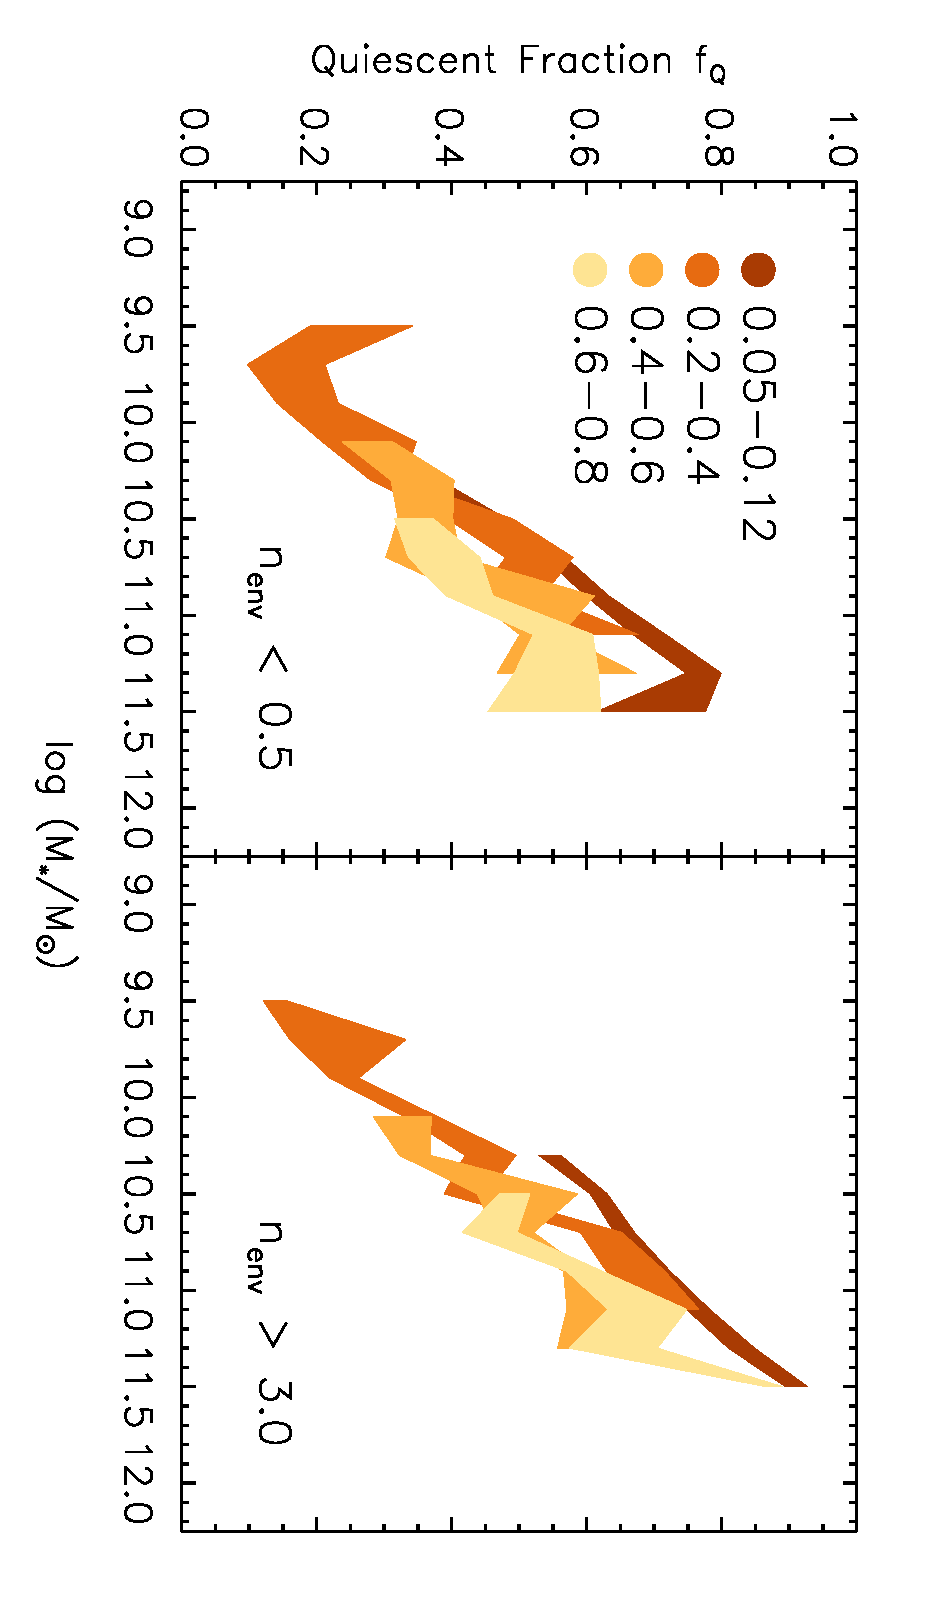
\epsfig{file=fig_qf_cylr2h25_thresh75_bin0_20_sdss_z0_05_0_12_primus_z0_2_1_0_lowenv0_5_highenv3_0_lit_primuszerr.eps, height=0.75\textwidth,angle=90}
        \caption{Evolution of the quiescent fraction $f_{\rm{Q}}$ for galaxies in low (left) and high (rights) density environments for $z < 0.8$. $f_{\rm{Q}}$s were calculated using the SMFs in Figure\ref{fig:smf}, as described in text. Darker shading indicates lower redshift and the width represents the standard jackknife uncertainty.}         \label{fig:qf}
    \end{center}
\end{figure*}
%%%%%%%%%%%%%%%%%%%%%%%%%%%%%%%%%%%%%%%%%%%%%%%%%%%%%%%%%%%%%%%%%%%%%%%%%%%%%%%%%%%%
% QUIESCENT FRACTION
%%%%%%%%%%%%%%%%%%%%%%%%%%%%%%%%%%%%%%%%%%%%%%%%%%%%%%%%%%%%%%%%%%%%%%%%%%%%%%%%%%%%
\section{Quiescent Fraction} \label{sec:qf_const}
The SMFs calculated in the previous section illustrate the stellar mass distribution of our galaxy population and its evolution over comic time. In this section, using the SMFs of our subsamples, we compare the quiescent and the star-forming populations by calculating the fraction of galaxies that have quenched their star-formation, the quiescent fraction. 

With the sufficient statistics available from SDSS and PRIMUS, we evaluate the quiescent fraction in bins of stellar mass and redshift for low and high density environments (Section \ref{sec:qfevol}). More specifically, by analyzing the quiescent fraction with respect to mass, redshift, and environment we are able to compare the quiescent fraction evolution in low and high density environments. Through this comparison, in Section \ref{sec:env_qf_evol}, we reveal the subtle environmental effects in quenching star formation that are often obscured by the underlying correlations among galactic properties such as color-mass and mass-density relations (\cite{Cooper:2010aa}). Furthermore by quantifying the environmental effects of star-formation quenching, we are able to provide constraints on the various proposed environmental quenching mechanisms, such as strangulation and ram-pressure stripping (\cite{McCarthy:2008aa}).
%%%%%%%%%%%%%%%%%%%%%%%%%%%%%%%%%%%%%%%%%%%%%%%%%%%%%%%%%%%%%%%%%%%%%%%%%%%%%%%%%%%%
% EVOLUTION OF THE QUIESCENT FRACTION
%%%%%%%%%%%%%%%%%%%%%%%%%%%%%%%%%%%%%%%%%%%%%%%%%%%%%%%%%%%%%%%%%%%%%%%%%%%%%%%%%%%%
\subsection{Evolution of the Quiescent Fraction} \label{sec:qfevol}
From the SMF number densities ($\Phi$) computed in the previous section, the quiescent fraction is computed as follows, 
\begin{equation}
f_{\rm{Q}} = \frac{\Phi_{Q}}{\Phi_{SF}+\Phi_{Q}}.
\end{equation}
$\Phi_{Q}$ and $\Phi_{SF}$ are the total number of galaxies per unit volume in stellar mass bin of $\Delta(\rm{log} \: \mathcal{M}) = 0.20 \: {\it dex}$ for the quiescent and star-forming subsamples, respectively (Equation \ref{eq:phi}). We compute $f_{\rm{Q}}$ for high and low density environments for all redshift bins as plotted in Figure \ref{fig:qf}, which shows the evolution of $f_{\rm{Q}}$ for high (right panel) and low (left panel) density environments. As in Figure \ref{fig:smf}, the evolution of the quiescent fraction over cosmic time is represented in the shading (darker with lower redshift) and the uncertainty is represented by the width. For the uncertainty in the quiescent fraction, we use the standard jackknife technique, following the same steps as the SMF uncertainty in Section \ref{sec:smfcalc}. 

Most noticeably in Figure \ref{fig:qf}, we find $f_{\rm{Q}}$ increases monotonically as a function of mass at all redshift bin and environment. In other words, for all subsamples, galaxies in higher mass bins are more likely to have quenched its star-formation. With the roughly linear correlation between galaxy SFR to galaxy color and morphology, we find that this trend reflects the well established color-mass and morphology-mass relations: more massive galaxies are more likely to be red or early-type (\cite{blanton09a}). 

Focusing on the redshift evolution of $f_{\rm{Q}}$, we find that for both environments $f_{\rm{Q}}$ increases as redshift decreases. For high density environment, this is analogous to the Butcher-Omeler Effect (\cite{Butcher:1984aa}), which states that galaxy populations in groups or clusters have higher $f_{\rm{blue}}$, or lower $f_{\rm{Q}}$, at higher redshift. For all environments, a larger portion of our galaxy population has quenched its star-formation over time. Coupled with the decline of SFR in the star-forming population (\cite{Noeske:2007aa}; \cite{cooper08a}), our results are in agreement with the observed decline of global star-formation in the universe (\cite{hopkins06a}). %Maybe Stacey et al. 2014 is relevant here? 

In addition, when we compare the stellar masses at which $f_{\rm{Q}} = 0.5$ for each subsample, the so-called $\mathcal{M}_{50-50}$, we find that this quantity decreases over cosmic time. This corresponds to the well-known mass-downsizing pattern in the literature (e.g. \cite{bundy06a}). Furthermore, the mass-downsizing trend observed in each of our environment subsample is consistent with the trend observed in zCOSMOS Redshift Survey for isolated and group galaxies (\cite{Iovino:2010aa}). %Remark on how the M_{50-50}? is lower for high environment f_{Q}, and that it generally increases with redshift. A trend also observed in the t_{5050} considerations.

Finally, we compare our $f_{\rm{Q}}$ results to previous $f_{\rm{Q}}$ (or $f_{\rm{red}}$) measurements with analogous environment classifications. For our lowest redshift bin, we find that our $f_{\rm{Q}}$ for low and high environments are consistent with previous SDSS $f_{\rm{Q}}$ (or $f_{\rm{red}}$) measurements as a function of environment. For example, \cite{Tinker:2011aa}, using a group-finding algorithm on the SDSS DR7, presents the relationship between $f_{\rm{Q}}$ and overdensity for galaxies within the mass range $\rm{log} \; \mathcal{M} = [9.8, 10.1]$. The \cite{Tinker:2011aa} $f_{\rm{Q}}$ at the lowest and highest overdensities, $f_{\rm{Q}} \sim 0.4$ and $f_{\rm{Q}} \sim 0.6$ respectively, are consistent with our $f_{\rm{Q}}$ for low and high density environment at the lower mass limit ($\rm{log} \; \mathcal{M} \sim 10.2$). 

At higher masses, our $f_{\rm{Q}}$ results are consistent with \cite{Baldry:2006aa}. \cite{Baldry:2006aa} uses project neighbor density environment measures ($\rm{log} \;  \Sigma$) to obtain $f_{\rm{Q}}(\mathcal{M})$ for a range of environmental densities. Although in these comparisons, the different environment measurements make direct comparisons unclear, at higher environments ($\rm{log} \; \Sigma > 0.2$ in \cite{Baldry:2006aa}) $f_{\rm{Q}}(\mathcal{M} \sim 10^{10.2} \mathcal{M}_{\odot}) \sim 0.6$ and $f_{\rm{Q}}(\mathcal{M} \sim 10^{11.5} \mathcal{M}_{\odot}) \sim 0.9$, in agreement our high density environment. Likewise, for lower environments ($\rm{log} \; \Sigma < -0.4$ in \cite{Baldry:2006aa}) $f_{\rm{Q}}(\mathcal{M} \sim 10^{10.2} \mathcal{M}_{\odot}) \sim 0.4$ and $f_{\rm{Q}}(\mathcal{M} \sim 10^{11.5} \mathcal{M}_{\odot}) \sim 0.8$, which also agree with our low density environment $f_{\rm{Q}}$. 

For $z > 0.2$, we compare our PRIMUS $f_{\rm{Q}}$ results to the $f_{\rm{red}}$ (or $1-f_{\rm{blue}}$) results from the zCOSMOS Redshift Survey (\cite{Iovino:2010aa}, \cite{Cucciati:2010aa}, \cite{Kovac:2014aa}), which covers a similar redshift range as PRIMUS. \cite{Iovino:2010aa}, \cite{Cucciati:2010aa}, and \cite{Kovac:2014aa} using a mass-complete galaxy sample derived from zCOSMOS and a group catalog, 3D local density contrast, and overdensity environment measurements, respectively, compare $f_{\rm{red}}$ with respect to environment. The $f_{\rm{blue}}$ for group and isolated galaxies from \cite{Iovino:2010aa} are generally inconsistent with our $1-f_{\rm{Q}}$ for high and low density environments. 

Similarly, $f_{\rm{red}}$ for high and low overdensities in \cite{Kovac:2014aa} are  greater overall than the PRIMUS $f_{\rm{Q}}$ values in high and low density environments. However, \cite{Kovac:2014aa} points out that there is a significant difference between classifying the quenched population using color and SFR. For their lower redshift bin ($0.1 < z < 0.4$) they find that their $f_{\rm{Q}}$ defined by color is greater than $f_{\rm{Q}}$ defined by SFR by roughly $0.2$. While for their higher redshift bin ($0.4 < z < 0.7$) they find a difference of $0.15-0.19$. Although the propagation of this difference for different environments is not explored in \cite{Kovac:2014aa}, if we naively account for the difference uniformly for $f_{\rm{red}}$ at all environments, the \cite{Kovac:2014aa} results in their lower redshift bin are generally consistent with our $f_{\rm{Q}}$ at high and low density environments. However, in their higher redshift bin even accounting for the difference in galaxy classification, \cite{Kovac:2014aa} finds a significantly higher $f_{\rm{Q}}$. 

We previously addressed that for both low and high density environments, $f_{\rm{Q}}$ increases as redshift decreases. This general trend is in good agreement with \cite{Iovino:2010aa}, which finds a similar increase in $1-f_{\rm{blue}}$ over cosmic time for $\mathcal{M} < 10^{10.9} \mathcal{M}_{\odot}$. However, in contrast to our $f_{\rm{Q}}$ redshift evolution, \cite{Kovac:2014aa} presents a notable decrease in $f_{\rm{red}}$ over cosmic time for low environment. Even for their galaxies in high density environments, \cite{Kovac:2014aa} finds no significant increase in $f_{\rm{red}}$ with cosmic time. 

The zCOSMOS results also find that $f_{\rm{red}}$ in high density environments are greater overall than in low density environments. The same trend is observed in the PRIMUS results and will be discussed in detail later in Section \ref{sec:env_qf_evol}. Another significant trend observed in the zCOSMOS results is the significant mass dependence of the $f_{\rm{red}}$ and $f_{\rm{blue}}$ evolution. \cite{Iovino:2010aa} by examining $f_{\rm{blue}}(z)$ in different mass bins for group and isolated galaxies find significantly larger $f_{\rm{blue}}$ evolution at lower masses. In fact, \cite{Iovino:2010aa} finds no evolution in $f_{\rm{blue}}$ for $\mathcal{M} > 10^{10.9} \mathcal{M}_{\odot}$ for both group and isolated galaxies over the redshift range $0.4 < z < 0.9$. On the other hand, in the lowest mass bin ($10^{10.0} \mathcal{M}_{\odot} < \mathcal{M} < 10^{10.5} \mathcal{M}_{\odot}$) \cite{Iovino:2010aa} finds $f_{\rm{blue}}(z \sim 0.4) - f_{\rm{blue}}(z \sim 0.2) \sim 0.2$ for isolated galaxies and  $f_{\rm{blue}}(z \sim 0.4) - f_{\rm{blue}}(z \sim 0.2) \sim 0.1$ for group galaxies. In contrast, in each of the panels of Figure \ref{fig:qf}, we qualitatively find little mass dependence on the $f_{\rm{Q}}$ evolution for either low or high density environments. However, due to the distinct stellar mass completeness limits imposed at each redshift bin of our sample, subtle effects such as the mass dependence of the $f_{\rm{Q}}$ evolution are difficult to discern. 

\begin{figure}
    \begin{center}
        \leavevmode
        \epsscale{1.0}
        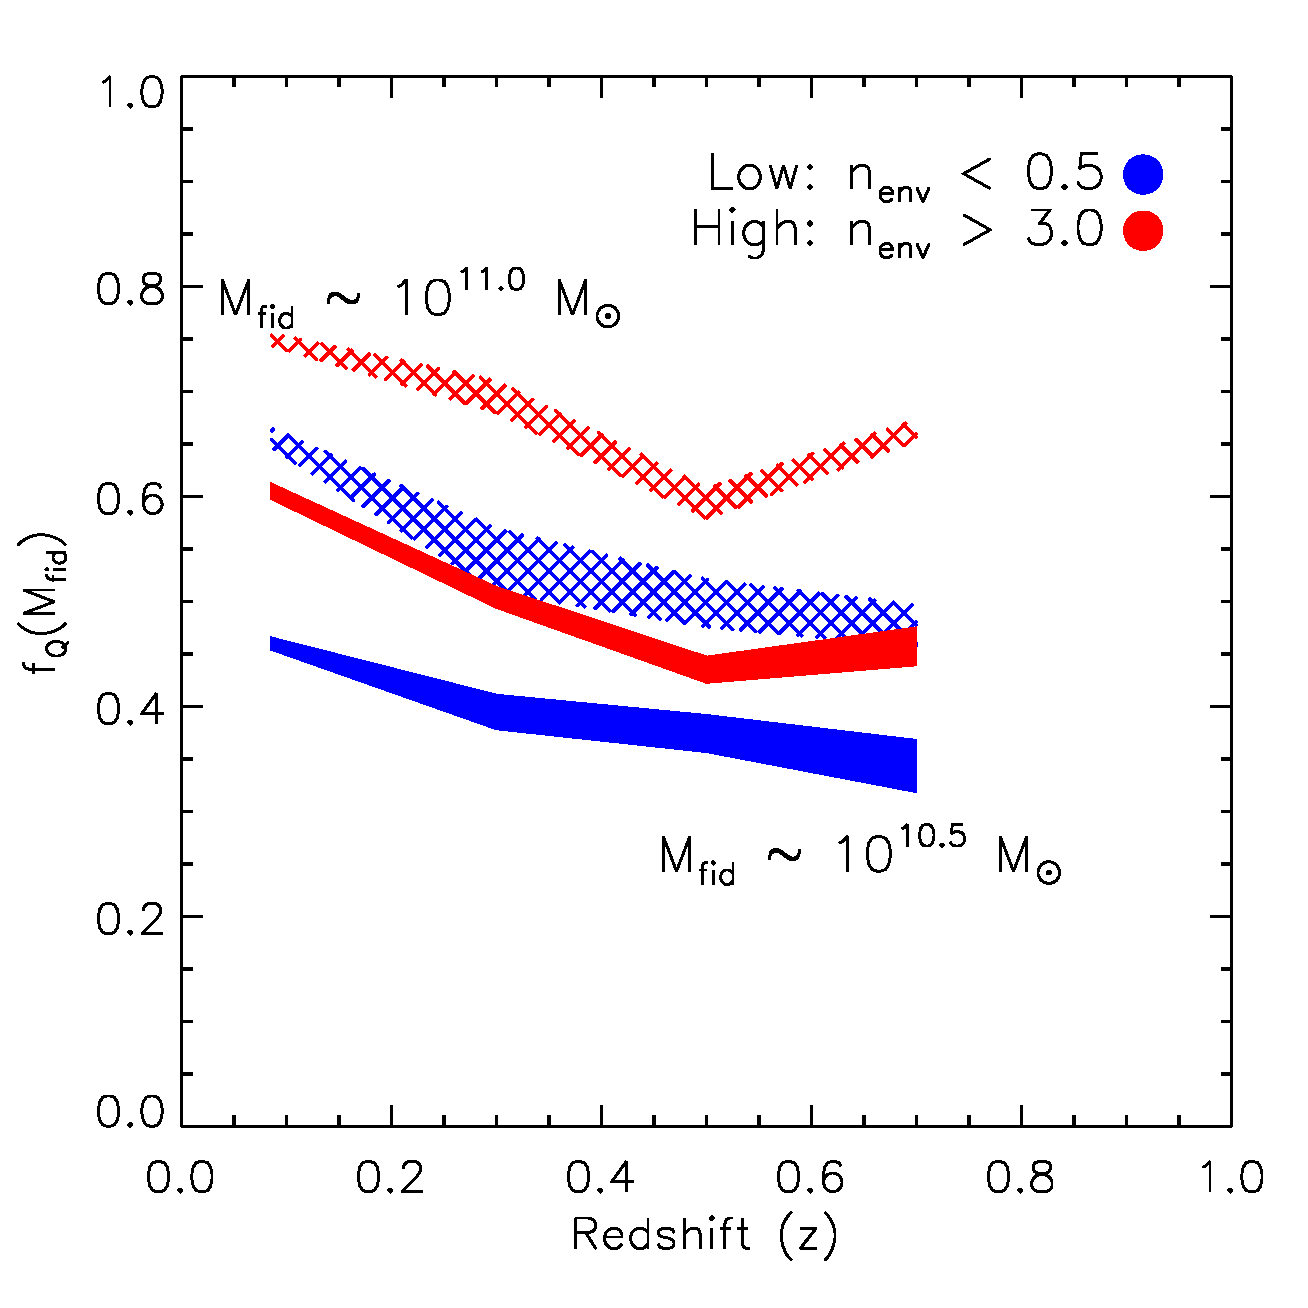
\epsfig{file=fig_qffit_cylr2h25_thresh75_bin0_20_sdss_z0_05_0_12_primus_z0_2_1_0_lowenv0_5_highenv3_0_fidmasscomp11_0_10_5_lit_primuszerr.eps, height=0.45\textwidth}
        \caption{The evolution of the quiescent fraction at fiducial mass, $f_{Q}(\mathcal{M}_{\rm{fid}})$, for low (blue) and high (red) density environments within the redshift range $z = 0.0 - 0.8$. We present the $f_{Q}(\mathcal{M}_{\rm{fid}})$ evolution for $\mathcal{M}_{\rm{fid}} = 10^{10.5} \mathcal{M}_\odot$ (solid fill) and $10^{11} \mathcal{M}_\odot$ (patterned fill) with the uncertainty of the best-fit parameter $b$ in Equation \ref{eq:qffit} represented by the width of the evolution. There is a significant increase in $f_{Q}(\mathcal{M}_{\rm{fid}})$ with decrease in redshift for both environments. In addition, over the entire redshift range, high density environment $f_{Q}(\mathcal{M}_{\rm{fid}})$ is greater than low density environment $f_{Q}(\mathcal{M}_{\rm{fid}})$. For the environment cut-offs ($n_{\rm{env}} < 0.5$ for low and $n_{\rm{env}} > 3.0$ for high), there is no significant difference in the slope of the evolution between the environments.}         \label{fig:qffit}
    \end{center}
\end{figure}

%%%%%%%%%%%%%%%%%%%%%%%%%%%%%%%%%%%%%%%%%%%%%%%%%%%%%%%%%%%%%%%%%%%%%%%%%%%%%%%%%%%%
% ENVIRONMENTAL EFFECTS ON THE QUIESCENT FRACTION EVOLUTION
%%%%%%%%%%%%%%%%%%%%%%%%%%%%%%%%%%%%%%%%%%%%%%%%%%%%%%%%%%%%%%%%%%%%%%%%%%%%%%%%%%%%
\subsection{Environmental Effects on the Quiescent Fraction Evolution} \label{sec:env_qf_evol}
In order to more quantitatively compare the $f_{\rm{Q}}$ evolution for different epochs and environments, we fit $f_{\rm{Q}}$ for each subsample to a power-law parameterization as a function of stellar mass, 
\begin{equation} \label{eq:qffit}
f_{\rm{Q}}(\mathcal{M}_{*}) = a \: \rm{log} \; \left(\frac{ \mathcal{M}_{*}}{\mathcal{M}_{\rm{fid}}} \right)+b,
\end{equation}
where $a$ and $b$ are best-fit parameters using {\em MPFIT} (\cite{Markwardt:2009aa}) and $\mathcal{M}_{\rm{fid}}$ represents the empirically selected fiducial mass within the stellar mass limits where there is a sufficiently large number of galaxies. We primarily focus on $\mathcal{M}_{\rm{fid}} = 10^{10.5} \: \mathcal{M}_{\odot}$. This fiducial mass serves to highlight and quantify the $f_{\rm{Q}}$ evolution for different redshifts. 

In Figure \ref{fig:qffit} we present the evolution of $f_{\rm{Q}}(\mathcal{M}_{\rm{fid}})$ from $z \sim 0.7$ to $\sim 0.1$ at low (blue) and high (red) density environments for $\mathcal{M}_{\rm{fid}} = 10^{10.5} \: \mathcal{M}_{\odot}$ (solid fill) and $10^{11} \: \mathcal{M}_{\odot}$ (pattern fill). Then in Figure \ref{fig:qffit_comp} we explore more stringent environment cut-offs for the high density environment (specified in the top right legend and represented by shading). In addition, we plot best-fit parameterization of $f_{\rm{red}}$ for high and low density environment from zCOSMOS, \cite{Iovino:2010aa} (square) and \cite{Kovac:2014aa} (triangle), and SDSS, \cite{Baldry:2006aa} (diamond). From \cite{Iovino:2010aa} we calculate $f_{\rm{red}} = 1-f_{\rm{blue}}$ using the best-fit $f_{\rm{blue}}$ from the mass bin $\mathcal{M} = 10^{10.3} - 10^{10.8} \mathcal{M}_{\odot}$. From \cite{Kovac:2014aa} we plot an estimated $f_{\rm{Q}}$ by applying the difference between SFR based and color based galaxy classifications to the best-fit $f_{\rm{red}}$ at $\mathcal{M} = 10^{10.5} \mathcal{M}_{\odot}$ for low ($\delta = 0.0$) and high density environment ($\delta = 1.5$). Similarly, from \cite{Baldry:2006aa} we plot $f_{\rm{Q}}$ derived from the best-fit $f_{\rm{red}}$ at $\mathcal{M} = 10^{10.5} \mathcal{M}_{\odot}$ for low ($\delta = 0.0$) and high density environment ($\delta = 1.0$).

\begin{table} 
  \caption{Best Fit Parameters for $f_{\rm{Q}}(\mathcal{M}_{*})$ Fit}
  \label{tab:bestfitparam}
  \begin{center}
    \leavevmode
    \begin{tabular}{lllll} \hline \hline              
    $z_1 < z < z_2$ &Environment        &a  &b  \\ \hline 
$0.05 < z< 0.12$ &$n_{\rm{env}} < 0.5$           &$0.3612 \pm 0.015$	&$0.482 \pm 0.006$                           \\
               &$n_{\rm{env}} > 3$            &18952                       &13387                           \\ 
                              &               &                       &                           \\ \hline
$0.2 < z <0.4$      &Low           &1158                    &3445                           \\
               &High            &817                    &1531                           \\
               &               &                       &                           \\ \hline
$0.4 < z < 0.6$      &Low           &1315                       &3390                           \\
               &High            &848                       &1499                           \\
               &               &                       &                           \\ \hline
$0.6 < z < 0.8$      &Low           &1158                       &2303                           \\
               &High            &900                       &1275                           \\
               &               &                       &                           \\ \hline
  \multicolumn{4}{l}{}                                             \\       
    \end{tabular} \par
    \end{center}
%    \bigskip 
    {\bf Notes}: Best fit parameters in Equation \ref{eq:qffit} for each subsample $f_{\rm{Q}}(\mathcal{M}_{*})$ in Figure \ref{fig:qf} for $\mathcal{M}_{\rm{fid}} = 10^{10.5} \mathcal{M}_{\odot}$.
\end{table}

\begin{figure}
    \begin{center}
        \leavevmode
        \epsscale{1.0}
        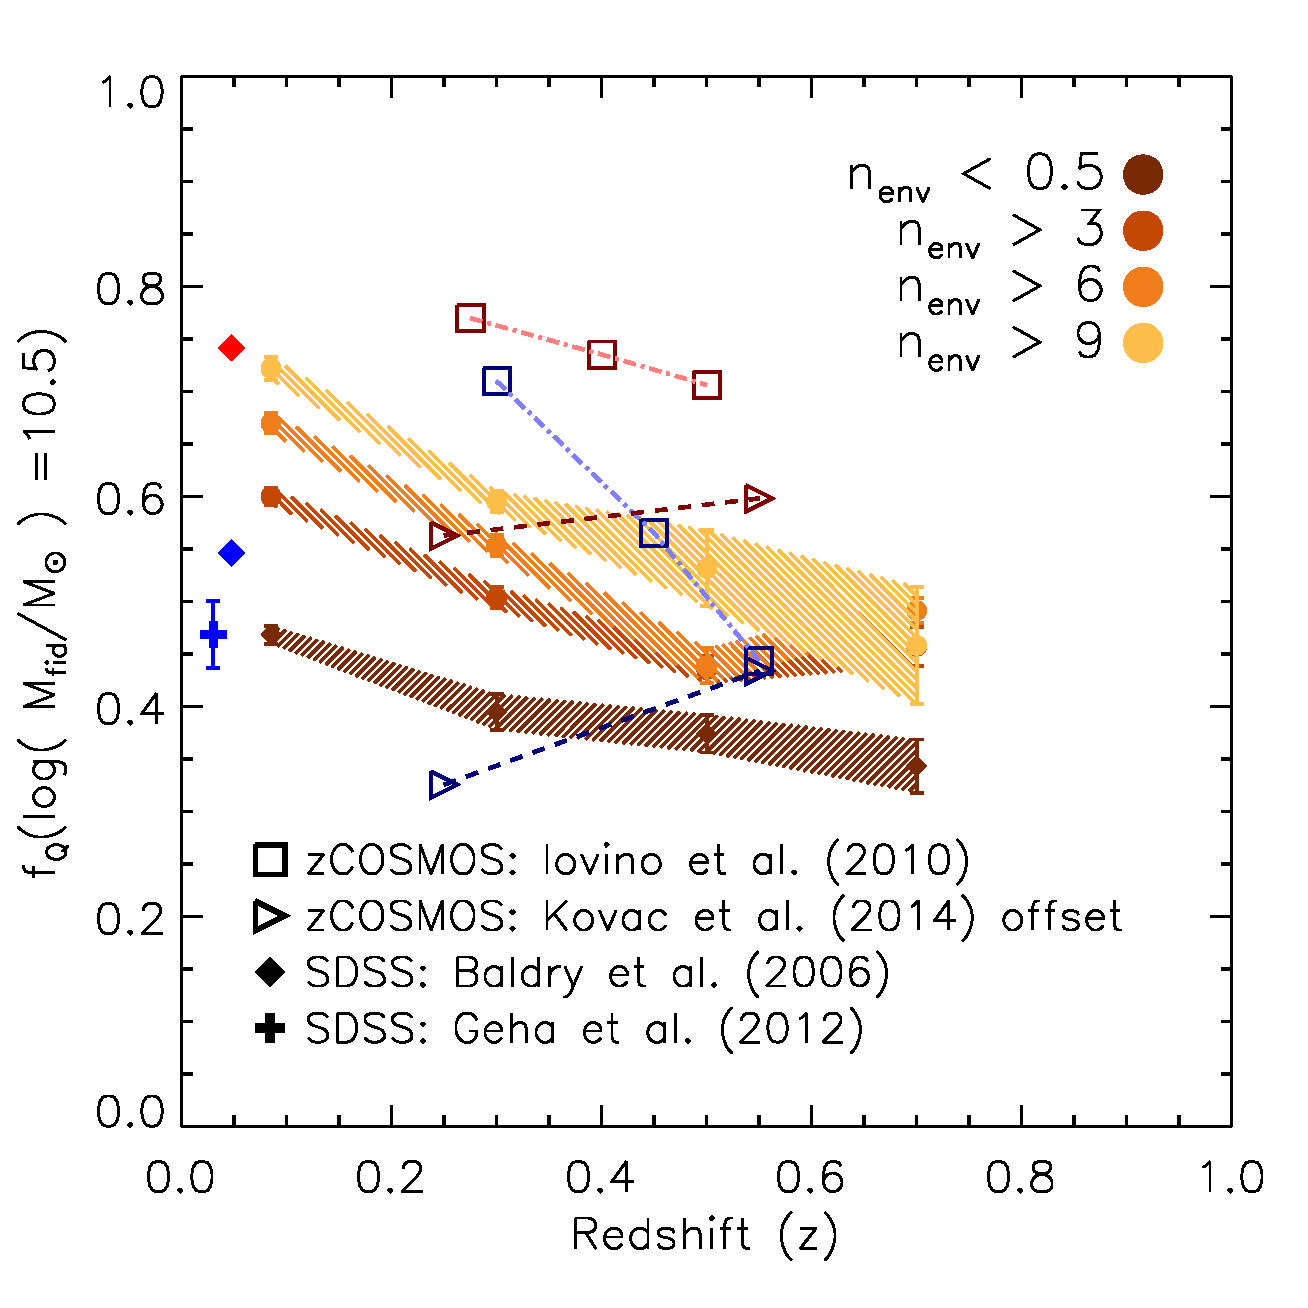
\epsfig{file=fig_qffit_cylr2h25_thresh75_bin0_20_sdss_z0_05_0_12_primus_z0_2_1_0_lowenv0_5_highenv3_0_fidmass10_5_lit_primuszerr_zcosmoscomp_envthresh_kovacoffset.eps, height=0.45\textwidth}
        \caption{$f_{\rm{Q}}(\mathcal{M}_{\rm{fid}}=10^{10.5} \mathcal{M}_\odot)$ evolution compared to $f_{\rm{red}}(\mathcal{M}_{*}=10^{10.5} \; \mathcal{M}_{\odot})$ in the literature: \cite{Iovino:2010aa} (square) and \cite{Kovac:2014aa} (triangle) from zCOSMOS and \cite{Baldry:2006aa} (diamond) from SDSS. These $f_{\rm{red}}$ values are calculated from the best-fit parameterizations presented in the respective works. High density environment is represented in red and low density environment is represented in blue. For \cite{Kovac:2014aa} we apply the offset between the color-based and SFR-based galaxy classification in order to plot the $f_{\rm{Q}}$ estimates. We also plot the $f_{\rm{Q}}(\mathcal{M}_{\rm{fid}} = 10^{10.5} \mathcal{M}_\odot)$ evolution of our sample with varying environment cut-offs specified on the top right. As in Figure \ref{fig:qffit} the width of the $f_{\rm{Q}}(\mathcal{M}_{\rm{fid}} = 10^{10.5} \mathcal{M}_\odot)$ evolution represent the uncertainty in the best-fit parameters of Equation \ref{eq:qffit}.}         \label{fig:qffit_comp}
    \end{center}
\end{figure}

Both Figure \ref{fig:qffit} and Figure \ref{fig:qffit_comp} illustrate that throughout the entire redshift range, high density environment has a significantly greater $f_{\rm{Q}}(\mathcal{M}_{\rm{fid}})$ than the lower density environment. This is in strong agreement with the zCOSMOS results from \cite{Cucciati:2010aa} and \cite{Kovac:2014aa} and suggests that galaxy populations in higher density environments at $z < 1.0$ have higher quenched fractions. As galaxy color serves as a proxy for SFR, our results support the existence of the color-density relation (\cite{Cucciati:2010aa}; \cite{Cooper:2010aa}) and debunk the suggestions that the color-density relation is a merely a reflection of the mass-density or morphology-density relation (\cite{Scodeggio:2009aa}, \cite{Tasca:2009aa}).  

In Figure \ref{fig:qffit}, for $\mathcal{M}_{\rm{fid}} = 10^{11} \mathcal{M}_\odot$, aside from an overall shift in $f_{\rm{Q}}(\mathcal{M}_{\rm{fid}})$ by $\sim 0.2$, we observe the same evolutionary trends. $f_{\rm{Q}}(\mathcal{M}_{\rm{fid}} = 10^{11}\mathcal{M}_{\odot})$ for both low and high density environments each increase by $\sim 0.2$ as redshift decreases from $\sim 0.7$ to $\sim 0.1$, keeping the slope of the $f_{\rm{Q}}(\mathcal{M}_{\rm{fid}})$ evolution the same. Evidently, increasing the fiducial mass to $10^{11} \mathcal{M}_{\odot}$ does not significantly alter the total evolution for either environments. 

The similarity of the evolutionary trends at $\mathcal{M}_{\rm{fid}} = 10^{10.5} \: \mathcal{M}_{\odot}$ and $10^{11} \: \mathcal{M}_{\odot}$ conflicts with \cite{Iovino:2010aa} who find contrasting $f_{\rm{Q}}$ evolutions at $\mathcal{M} \sim 10^{11.0} \mathcal{M}_{\odot}$ and $\mathcal{M} \sim 10^{10.5} \mathcal{M}_{\odot}$,  for both group and isolated galaxies. In fact at their highest mass bin ($10^{10.9} - 10^{11.4} \mathcal{M}_{\odot}$), \cite{Iovino:2010aa} find no evolution for both environments: $f_{\rm{blue}}$ remains constant at $\sim 0.1$ within $z = 0.3 - 0.8$ for both group and isolated galaxy populations. Meanwhile in their mass bin most comparable to our $\mathcal{M}_{\rm{fid}} = 10^{10.5} \mathcal{M}_{\odot}$, they present an evolution of $\Delta f_{\rm{red}} \sim 0.1$ over $z = 0.5$ to $0.25$ for group galaxies and $\Delta f_{\rm{red}} \sim 0.3$ over $z = 0.55$ to $0.3$. Furthermore, while we find that the $f_{\rm{Q}}(z)_{\rm{high}} - f_{\rm{Q}}(z)_{\rm{low}}$ remains relatively constant at $\sim 0.1$ over the redshift range for both fiducial masses, \cite{Iovino:2010aa} finds $f_{\rm{blue}}(z)_{ \rm{isolated}} - f_{\rm{blue}}(z)_{\rm{group}}$ is much more significant at $\mathcal{M} \sim 10^{10.5} \mathcal{M}_{\odot}$ than at $\mathcal{M} \sim 10^{11} \mathcal{M}_{\odot}$, where they find no difference. 

zCOSMOS results find a clear mass dependence in the $f_{\rm{blue}}$ evolution; however, the consistency in evolutionary trends when the fiducial mass is changed reveal that our $f_{\rm{Q}}$ evolution exhibits little mass dependence. Although our sample from SDSS and PRIMUS provides significantly larger statistics, due to the limited mass ranges probed in our mass-complete sample (e.g. $\mathcal{M} > 10^{10.5} \mathcal{M}_{\odot}$ for our $z \sim 0.7$ bin) it is difficult to dismiss the mass dependence observed in the zCOSMOS results.

Another trend we observe in both Figure \ref{fig:qffit} Figure \ref{fig:qffit_comp}, is that for both environments $f_{\rm{Q}}(\mathcal{M}_{\rm{fid}})$ increases as redshift decreases. This highlights the general increase of $f_{\rm{Q}}(\mathcal{M})$ as redshift decreases noted earlier. More importantly, by fitting our $f_{\rm{Q}}$ evolution and obtaining the value at the fiducial mass, we are able to quantify the total evolution of $f_{\rm{Q}}$ for both low and high density environments through $f_{\rm{Q}}(\mathcal{M}_{\rm{fid}}, z \sim 0.1) - f_{\rm{Q}}(\mathcal{M}_{\rm{fid}}, z \sim 0.7)$ for both environments. In Figure \ref{fig:qffit}, we find that $f_{\rm{Q}}$ evolves by a similar amount for both environments. 

Considering that fixed aperture definition of environment is susceptible to contamination due to PRIMUS redshift errors, in Figure \ref{fig:qffit_comp}, we consider more stringent classification of high density environments extending the cut-off to $n_{\rm{env}} > 6, 9$. A more stringent classification significantly increases the $f_{\rm{Q}}(\mathcal{M}_{\rm{fid}})$ overall. The decrease in sample size that accompanies a purer high environment sample also increase the uncertainties. More importantly, a purer high environment classification reveals a more significant environment dependence of the $f_{\rm{Q}}$ evolution. With a purer the high environment classification, we find a steeper slope in the $f_{\rm{Q}}$ and a greater total $f_{\rm{Q}}$ evolution. From $ z \sim 0.7$, for the low density environment ($n_{\rm{env}} < 0.5$) $f_{\rm{Q}}$ increases by roughly $0.1$. At the highest environments, $f_{\rm{Q}}$ increases by roughly $0.25$. Therefore, the total evolution of $f_{\rm{Q}}(\mathcal{M}_{\rm{fid}})$ from $z \sim 0.7$ to $\sim 0.1$ show moderate environment dependence.

An environment dependence of the $f_{\rm{Q}}$ evolution is also observed in \cite{Iovino:2010aa} - also plotted in Figure \ref{fig:qffit_comp}. However, in addition to a much more pronounced distinction between the group and isolated $f_{\rm{Q}}$ evolution, they find the opposite environment dependence. Unlike our results, which find a greater $f_{\rm{Q}}$ evolution at higher density environments, \cite{Iovino:2010aa} finds a much greater evolution for isolated galaxies. 

\cite{Kovac:2014aa} finds a similar environment dependence on the total $f_{\rm{Q}}$ evolution to our results, with a greater $f_{\rm{Q}}$ evolution for high density environments. Unfortunately, contrary to our results, \cite{Kovac:2014aa} finds that $f_{\rm{Q}}$ decreases for both environments over cosmic time. The negative slope of the $f_{\rm{Q}}$ evolution is enhanced in Figure \ref{fig:qffit_comp} due to the galaxy classification correction we impose. However even without the correction (not shown), in their best-fit values, \cite{Kovac:2014aa} finds a decreasing $f_{\rm{Q}}$ evolution. 
%Discuss possible reasons for the difference between zCOSMOS results and our results. Point out the sample sizes and square degree coverage. 
% Kovac: 1.7 deg^2, 0.1 < z < 0.4 2340 and 0.4 < z < 0.7 2448. Most of the data points have errors of +/- 0.1, at least +/-0.05
% Iovino: 1.7 deg^2  617 galaxies in 10.3 < M < 10.8 and 0.1 < z < 0.6. Errors are +/1 0.1

Many physical mechanisms have been proposed to explain the quenching of star-formation observed in our universe. Often star-formation quenching is classified into two distinct mechanisms: mass-dependent and environment dependent mechanisms (\cite{Baldry:2006aa}; \cite{Peng:2010aa}). From the mass-dependence presented in all $f_{\rm{Q}}$ in Figure \ref{fig:qf}, we concur that galaxy stellar mass plays a significant role in quenching. Furthermore, since $f_Q$ in high density environments is always greater than $f_Q$ in low density environments, our results also reflect the environment dependence in quenching. %However, in many of the proposed environment dependent quenching mechanisms, the quenching time scale is proposed to decrease. This would result in an increase in the quenched fraction that's faster than the increase in low density environment $f_Q$. We find that this is not the case. % What does this have to say about physical processes in groups and clusters that affect quenching?

%%%%%%%%%%%%%%%%%%%%%%%%%%%%%%%%%%%%%%%%%%%%%%%%%%%%%%%%%%%%%%%%%%%%%%%%%%%%%%%%%%%%
% SUMMARY
%%%%%%%%%%%%%%%%%%%%%%%%%%%%%%%%%%%%%%%%%%%%%%%%%%%%%%%%%%%%%%%%%%%%%%%%%%%%%%%%%%%%
\section{Summary} \label{sec:summary}
Using a stellar mass complete galaxy sampled derived from SDSS and PRIMUS accompanied by a consistently measured galaxy environment from robust spectroscopic redshifts, we measure the stellar mass functions for star-forming and quiescent in low and high density environments over the redshift range $z < 0.8$. From these stellar mass functions, we compare the proportion of quiescent galaxies within the subsamples by computing quiescent fraction for each of them. Afterwards, in order to better quantify the evolution of the quiescent fraction over cosmic time, we fit our quiescent fraction anchored at a fiducial mass. From our analyses we find the following notable results. 

\begin{enumerate}
	\item By noting the SMF evolution for each of our subsamples, we loosely trace the evolutionary tracks our galaxy population tracing the general evolutionary tracks of quenching mechanisms and galaxies infalling into high density environments. 
	\item From the SMFs, we find that our galaxy population in high density environments, both star-forming and quiescent, have a higher median mass, thus confirming the mass density relation and mass-segregation in different environments.
	\item In all of our subsamples, we find a clear mass dependence in $f_{\rm{Q}}$. $f_{\rm{Q}}$ increases monotonically with galaxy stellar mass. 
	\item Both from the $f_{\rm{Q}}$ evolution and $f_{\rm{Q}}(\mathcal{M}_{\rm{fid}})$ values, $f_{\rm{Q}}$ increases with redshift. 
	\item We conclude, by fitting our $f_{\rm{Q}}$, that $f_{\rm{Q}}$ in high density environments is greater than $f_{\rm{Q}}$ in low density environments regardless of mass and redshift. This result confirms the environmental dependence of quenching mechanisms stated previously in literature. 
	\item Comparison of the $f_{\rm{Q}}(\mathcal{M}_{\rm{fid}})$ evolution for high and low density environments that the total evolution has a moderate dependence on environment. 
\end{enumerate}

%  demonstrate that the quiescent fraction increases over cosmic time for $ z < 0.8$, regardless of environment. During this epoch the quiescent fraction in high density environments is consistently greater than the quiescent fraction in low density environments. Furthermore, when we fit the quiescent fraction at a fiducial mass ($\mathcal{M}_{\rm{fid}}$), we find that the evolution of the quiescent fraction from $z \sim 0.8$ to $z \sim 0.1$ is similar for high and low density environments. 


We thank people and funding...
%
% References
%
\bibliography{PRIMUS}

\appendix
\begin{table*} %Will contain much more information on environments. 
  \caption{Environment Defining Aperture Dimensions}
  \label{tab:aperture}
  \begin{center}
    \leavevmode
    \begin{tabular}{llllll} \hline \hline              
  Radius (Mpc)          &Height (Mpc)      & Edge Effect Cutoff &High Env (galaxies) &Low Env (galaxies) \\ \hline 
  1.0 &50 & 80\% & 1.5 & 0.0          \\
  2.0 &50 & 75\% & 4.0 & 0.0          \\ \hline
  \multicolumn{5}{l}{}                                             \\       
    \end{tabular}
  \end{center}
\end{table*}

\begin{figure*}
    \begin{center}
        \leavevmode
        \epsscale{1.0}
        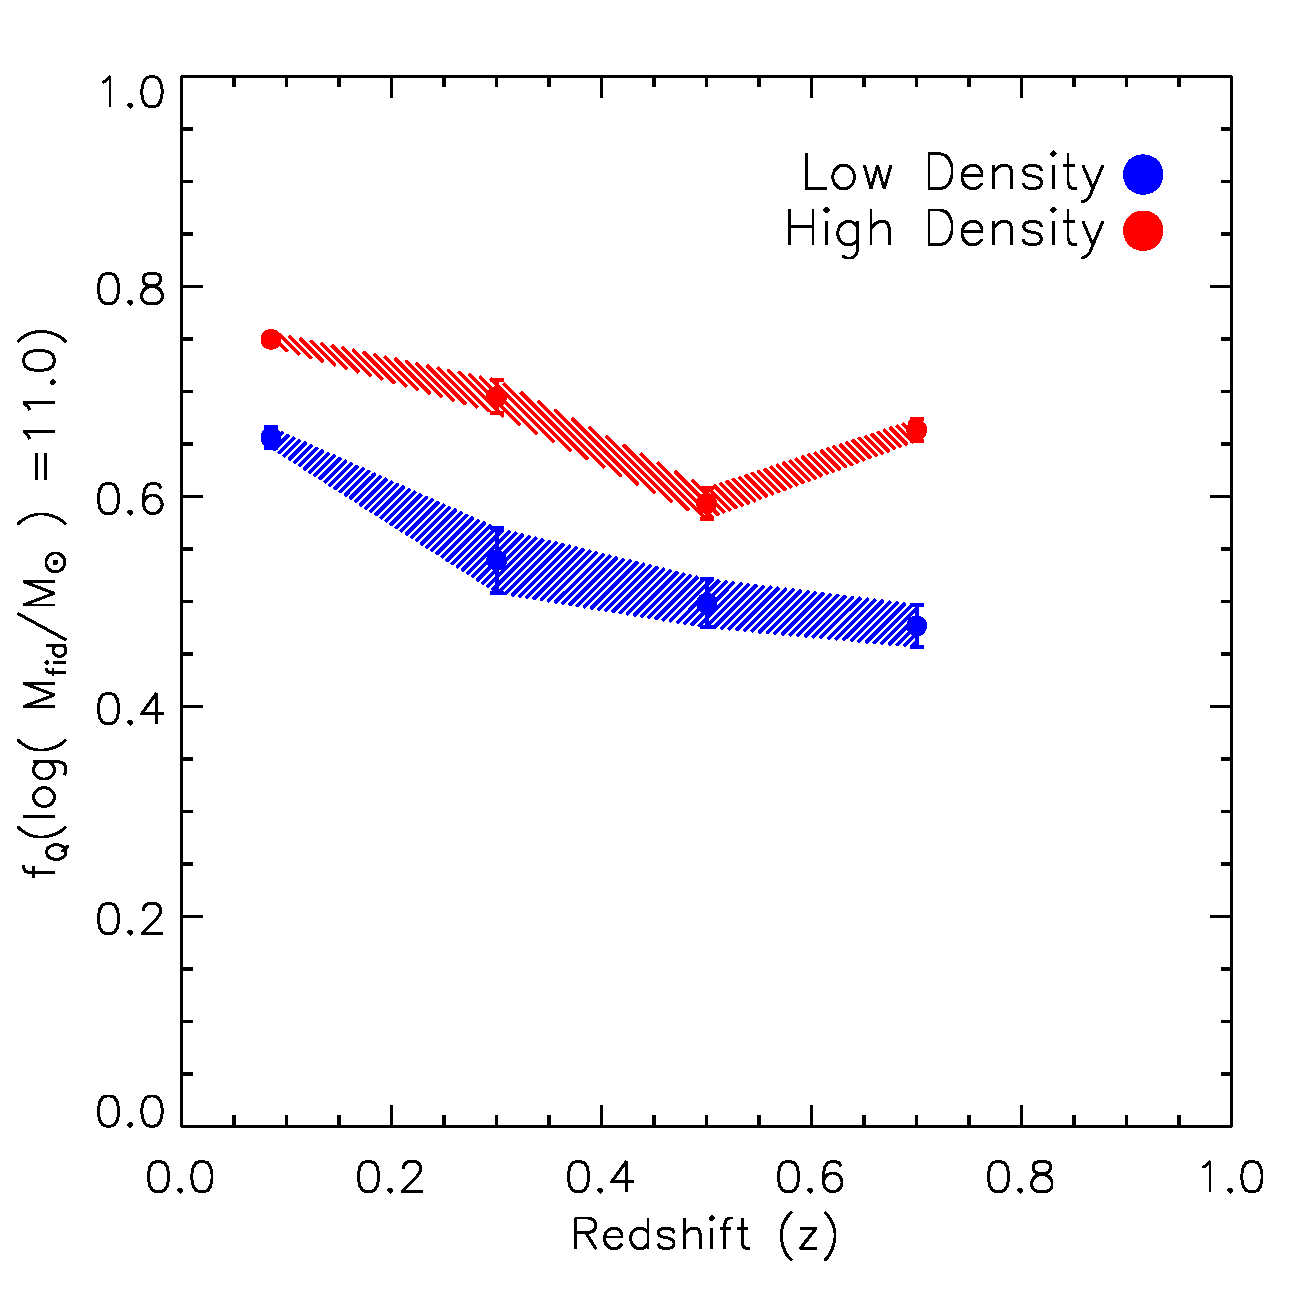
\epsfig{file=fig_qffit_cylr2h25_thresh75_bin0_20_sdss_z0_05_0_12_primus_z0_2_1_0_lowenv0_5_highenv3_0_fidmass11_0_lit_primuszerr.eps, height=0.45\textwidth}
        \caption{The evolution of the quiescent fraction at fiducial mass, $f_{Q}(\mathcal{M}_{\rm{fid}} = 10^{10.5} \mathcal{M}_\odot)$, for low (square) and high (circle) density environments within the redshift range $z = 0.0 - 0.8$.}      
    \end{center}
\end{figure*}

\begin{figure*}
    \begin{center}
        \leavevmode
        \epsscale{1.0}
        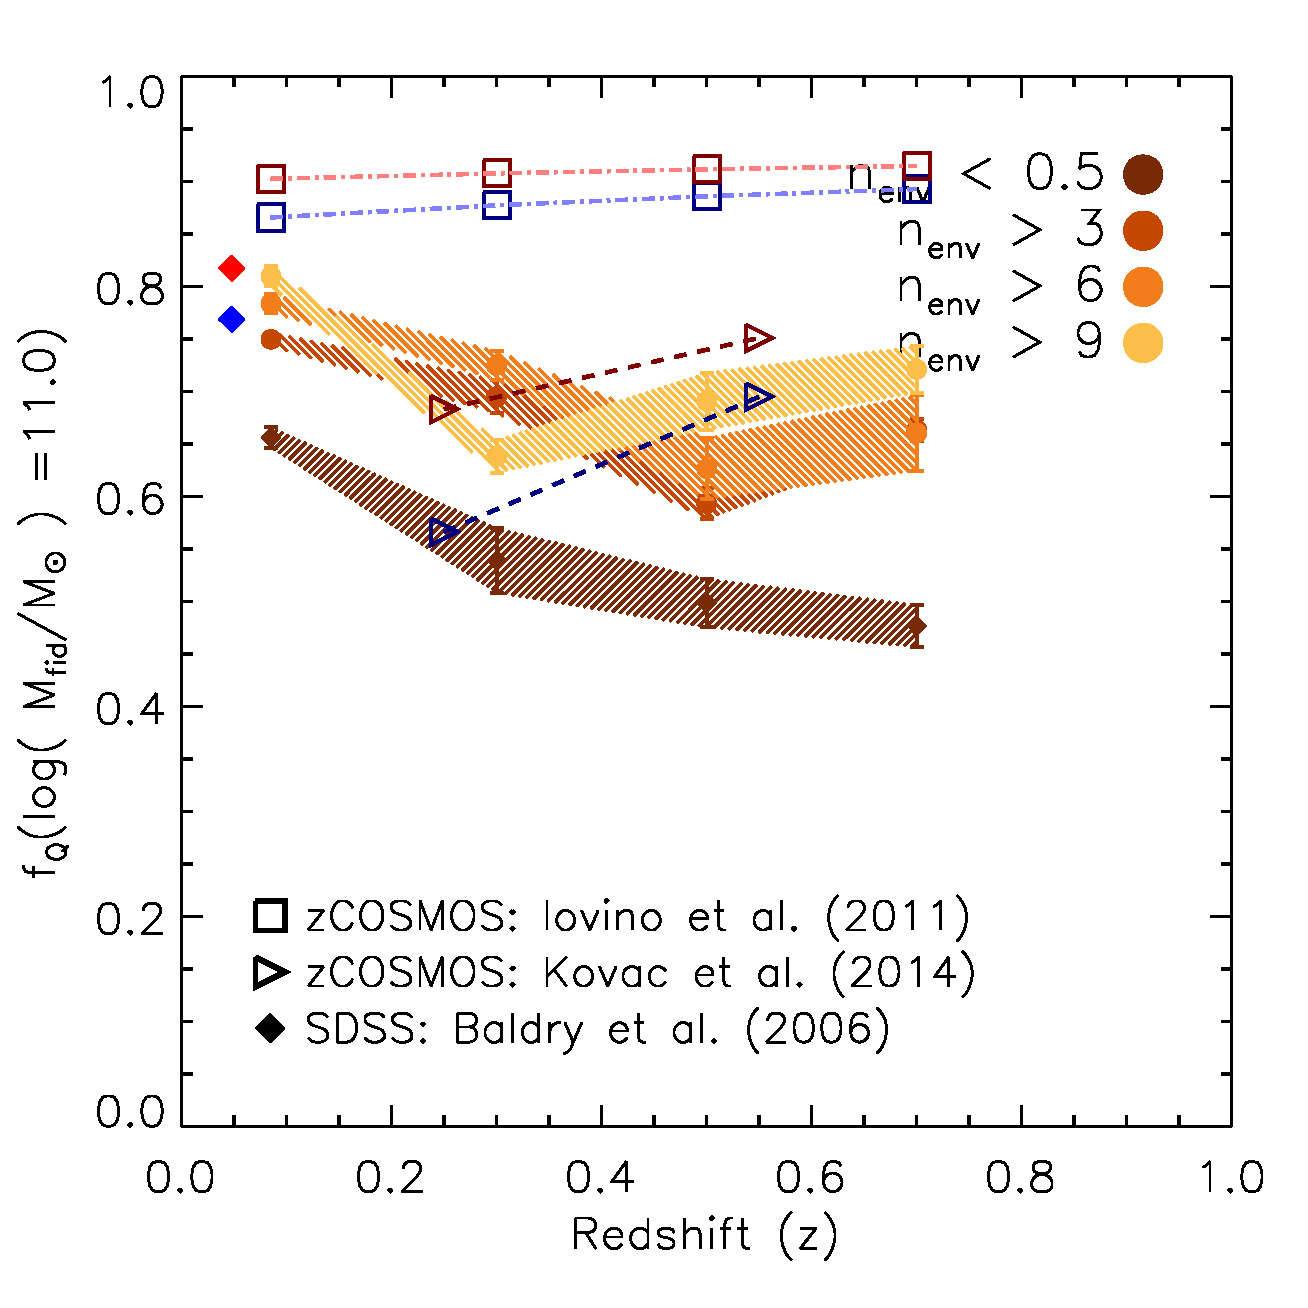
\epsfig{file=fig_qffit_cylr2h25_thresh75_bin0_20_sdss_z0_05_0_12_primus_z0_2_1_0_lowenv0_5_highenv3_0_fidmass11_0_lit_primuszerr_zcosmoscomp_envthresh_kovacoffset.eps, height=0.45\textwidth}
        \caption{The evolution of the quiescent fraction at fiducial mass, $f_{Q}(\mathcal{M}_{\rm{fid}} = 10^{10.5} \mathcal{M}_\odot)$, for low (square) and high (circle) density environments within the redshift range $z = 0.0 - 0.8$.}
    \end{center}
\end{figure*}

\end{document}